% Options for packages loaded elsewhere
\PassOptionsToPackage{unicode}{hyperref}
\PassOptionsToPackage{hyphens}{url}
\PassOptionsToPackage{dvipsnames,svgnames,x11names}{xcolor}
%
\documentclass[
  ignorenonframetext,
]{beamer}
\usepackage{pgfpages}
\setbeamertemplate{caption}[numbered]
\setbeamertemplate{caption label separator}{: }
\setbeamercolor{caption name}{fg=normal text.fg}
\beamertemplatenavigationsymbolsempty
% Prevent slide breaks in the middle of a paragraph
\widowpenalties 1 10000
\raggedbottom

\usepackage{amsmath,amssymb}
\usepackage{iftex}
\ifPDFTeX
  \usepackage[T1]{fontenc}
  \usepackage[utf8]{inputenc}
  \usepackage{textcomp} % provide euro and other symbols
\else % if luatex or xetex
  \usepackage{unicode-math}
  \defaultfontfeatures{Scale=MatchLowercase}
  \defaultfontfeatures[\rmfamily]{Ligatures=TeX,Scale=1}
\fi
\usepackage{lmodern}
\usetheme[]{AnnArbor}
\usecolortheme{dolphin}
\usefonttheme{structurebold}
\ifPDFTeX\else  
    % xetex/luatex font selection
\fi
% Use upquote if available, for straight quotes in verbatim environments
\IfFileExists{upquote.sty}{\usepackage{upquote}}{}
\IfFileExists{microtype.sty}{% use microtype if available
  \usepackage[]{microtype}
  \UseMicrotypeSet[protrusion]{basicmath} % disable protrusion for tt fonts
}{}
\makeatletter
\@ifundefined{KOMAClassName}{% if non-KOMA class
  \IfFileExists{parskip.sty}{%
    \usepackage{parskip}
  }{% else
    \setlength{\parindent}{0pt}
    \setlength{\parskip}{6pt plus 2pt minus 1pt}}
}{% if KOMA class
  \KOMAoptions{parskip=half}}
\makeatother
\usepackage{xcolor}
\newif\ifbibliography
\setlength{\emergencystretch}{3em} % prevent overfull lines
\setcounter{secnumdepth}{-\maxdimen} % remove section numbering

\usepackage{color}
\usepackage{fancyvrb}
\newcommand{\VerbBar}{|}
\newcommand{\VERB}{\Verb[commandchars=\\\{\}]}
\DefineVerbatimEnvironment{Highlighting}{Verbatim}{commandchars=\\\{\}}
% Add ',fontsize=\small' for more characters per line
\usepackage{framed}
\definecolor{shadecolor}{RGB}{241,243,245}
\newenvironment{Shaded}{\begin{snugshade}}{\end{snugshade}}
\newcommand{\AlertTok}[1]{\textcolor[rgb]{0.68,0.00,0.00}{#1}}
\newcommand{\AnnotationTok}[1]{\textcolor[rgb]{0.37,0.37,0.37}{#1}}
\newcommand{\AttributeTok}[1]{\textcolor[rgb]{0.40,0.45,0.13}{#1}}
\newcommand{\BaseNTok}[1]{\textcolor[rgb]{0.68,0.00,0.00}{#1}}
\newcommand{\BuiltInTok}[1]{\textcolor[rgb]{0.00,0.23,0.31}{#1}}
\newcommand{\CharTok}[1]{\textcolor[rgb]{0.13,0.47,0.30}{#1}}
\newcommand{\CommentTok}[1]{\textcolor[rgb]{0.37,0.37,0.37}{#1}}
\newcommand{\CommentVarTok}[1]{\textcolor[rgb]{0.37,0.37,0.37}{\textit{#1}}}
\newcommand{\ConstantTok}[1]{\textcolor[rgb]{0.56,0.35,0.01}{#1}}
\newcommand{\ControlFlowTok}[1]{\textcolor[rgb]{0.00,0.23,0.31}{\textbf{#1}}}
\newcommand{\DataTypeTok}[1]{\textcolor[rgb]{0.68,0.00,0.00}{#1}}
\newcommand{\DecValTok}[1]{\textcolor[rgb]{0.68,0.00,0.00}{#1}}
\newcommand{\DocumentationTok}[1]{\textcolor[rgb]{0.37,0.37,0.37}{\textit{#1}}}
\newcommand{\ErrorTok}[1]{\textcolor[rgb]{0.68,0.00,0.00}{#1}}
\newcommand{\ExtensionTok}[1]{\textcolor[rgb]{0.00,0.23,0.31}{#1}}
\newcommand{\FloatTok}[1]{\textcolor[rgb]{0.68,0.00,0.00}{#1}}
\newcommand{\FunctionTok}[1]{\textcolor[rgb]{0.28,0.35,0.67}{#1}}
\newcommand{\ImportTok}[1]{\textcolor[rgb]{0.00,0.46,0.62}{#1}}
\newcommand{\InformationTok}[1]{\textcolor[rgb]{0.37,0.37,0.37}{#1}}
\newcommand{\KeywordTok}[1]{\textcolor[rgb]{0.00,0.23,0.31}{\textbf{#1}}}
\newcommand{\NormalTok}[1]{\textcolor[rgb]{0.00,0.23,0.31}{#1}}
\newcommand{\OperatorTok}[1]{\textcolor[rgb]{0.37,0.37,0.37}{#1}}
\newcommand{\OtherTok}[1]{\textcolor[rgb]{0.00,0.23,0.31}{#1}}
\newcommand{\PreprocessorTok}[1]{\textcolor[rgb]{0.68,0.00,0.00}{#1}}
\newcommand{\RegionMarkerTok}[1]{\textcolor[rgb]{0.00,0.23,0.31}{#1}}
\newcommand{\SpecialCharTok}[1]{\textcolor[rgb]{0.37,0.37,0.37}{#1}}
\newcommand{\SpecialStringTok}[1]{\textcolor[rgb]{0.13,0.47,0.30}{#1}}
\newcommand{\StringTok}[1]{\textcolor[rgb]{0.13,0.47,0.30}{#1}}
\newcommand{\VariableTok}[1]{\textcolor[rgb]{0.07,0.07,0.07}{#1}}
\newcommand{\VerbatimStringTok}[1]{\textcolor[rgb]{0.13,0.47,0.30}{#1}}
\newcommand{\WarningTok}[1]{\textcolor[rgb]{0.37,0.37,0.37}{\textit{#1}}}

\providecommand{\tightlist}{%
  \setlength{\itemsep}{0pt}\setlength{\parskip}{0pt}}\usepackage{longtable,booktabs,array}
\usepackage{calc} % for calculating minipage widths
\usepackage{caption}
% Make caption package work with longtable
\makeatletter
\def\fnum@table{\tablename~\thetable}
\makeatother
\usepackage{graphicx}
\makeatletter
\def\maxwidth{\ifdim\Gin@nat@width>\linewidth\linewidth\else\Gin@nat@width\fi}
\def\maxheight{\ifdim\Gin@nat@height>\textheight\textheight\else\Gin@nat@height\fi}
\makeatother
% Scale images if necessary, so that they will not overflow the page
% margins by default, and it is still possible to overwrite the defaults
% using explicit options in \includegraphics[width, height, ...]{}
\setkeys{Gin}{width=\maxwidth,height=\maxheight,keepaspectratio}
% Set default figure placement to htbp
\makeatletter
\def\fps@figure{htbp}
\makeatother
% definitions for citeproc citations
\NewDocumentCommand\citeproctext{}{}
\NewDocumentCommand\citeproc{mm}{%
  \begingroup\def\citeproctext{#2}\cite{#1}\endgroup}
\makeatletter
 % allow citations to break across lines
 \let\@cite@ofmt\@firstofone
 % avoid brackets around text for \cite:
 \def\@biblabel#1{}
 \def\@cite#1#2{{#1\if@tempswa , #2\fi}}
\makeatother
\newlength{\cslhangindent}
\setlength{\cslhangindent}{1.5em}
\newlength{\csllabelwidth}
\setlength{\csllabelwidth}{3em}
\newenvironment{CSLReferences}[2] % #1 hanging-indent, #2 entry-spacing
 {\begin{list}{}{%
  \setlength{\itemindent}{0pt}
  \setlength{\leftmargin}{0pt}
  \setlength{\parsep}{0pt}
  % turn on hanging indent if param 1 is 1
  \ifodd #1
   \setlength{\leftmargin}{\cslhangindent}
   \setlength{\itemindent}{-1\cslhangindent}
  \fi
  % set entry spacing
  \setlength{\itemsep}{#2\baselineskip}}}
 {\end{list}}
\usepackage{calc}
\newcommand{\CSLBlock}[1]{\hfill\break\parbox[t]{\linewidth}{\strut\ignorespaces#1\strut}}
\newcommand{\CSLLeftMargin}[1]{\parbox[t]{\csllabelwidth}{\strut#1\strut}}
\newcommand{\CSLRightInline}[1]{\parbox[t]{\linewidth - \csllabelwidth}{\strut#1\strut}}
\newcommand{\CSLIndent}[1]{\hspace{\cslhangindent}#1}

\usepackage{booktabs}
\usepackage{longtable}
\usepackage{array}
\usepackage{multirow}
\usepackage{wrapfig}
\usepackage{float}
\usepackage{colortbl}
\usepackage{pdflscape}
\usepackage{tabu}
\usepackage{threeparttable}
\usepackage{threeparttablex}
\usepackage[normalem]{ulem}
\usepackage{makecell}
\usepackage{xcolor}

% logo
\titlegraphic{
\includegraphics[width=4cm]{../000_logos/logo-blue-vertical}}
\logo{\ifnum\thepage>1
\includegraphics[width=0.5cm]{../000_logos/logo-blue-vertical}\fi}

% UMNG: Manual de image institucional

% Colors

% Umng
\definecolor{yellow}{HTML}{fdc600}
\definecolor{red}{HTML}{ee2a24}

% Estudios a Distancia
\definecolor{blue1}{HTML}{12245b}
\definecolor{blue2}{HTML}{767ca6}
\definecolor{blue3}{HTML}{cad2ec}

% Modify items
\setbeamercolor{palette primary}{bg=blue3}
\setbeamercolor{palette tertiary}{bg=blue1}
\setbeamercolor{frametitle}{bg=yellow}

% Hyperlinks
\hypersetup{
  linkcolor=red,
  citecolor=red
}

\makeatletter
\@ifpackageloaded{caption}{}{\usepackage{caption}}
\AtBeginDocument{%
\ifdefined\contentsname
  \renewcommand*\contentsname{Table of contents}
\else
  \newcommand\contentsname{Table of contents}
\fi
\ifdefined\listfigurename
  \renewcommand*\listfigurename{List of Figures}
\else
  \newcommand\listfigurename{List of Figures}
\fi
\ifdefined\listtablename
  \renewcommand*\listtablename{List of Tables}
\else
  \newcommand\listtablename{List of Tables}
\fi
\ifdefined\figurename
  \renewcommand*\figurename{Figure}
\else
  \newcommand\figurename{Figure}
\fi
\ifdefined\tablename
  \renewcommand*\tablename{Table}
\else
  \newcommand\tablename{Table}
\fi
}
\@ifpackageloaded{float}{}{\usepackage{float}}
\floatstyle{ruled}
\@ifundefined{c@chapter}{\newfloat{codelisting}{h}{lop}}{\newfloat{codelisting}{h}{lop}[chapter]}
\floatname{codelisting}{Listing}
\newcommand*\listoflistings{\listof{codelisting}{List of Listings}}
\makeatother
\makeatletter
\makeatother
\makeatletter
\@ifpackageloaded{caption}{}{\usepackage{caption}}
\@ifpackageloaded{subcaption}{}{\usepackage{subcaption}}
\makeatother

\ifLuaTeX
\usepackage[bidi=basic]{babel}
\else
\usepackage[bidi=default]{babel}
\fi
\babelprovide[main,import]{english}
% get rid of language-specific shorthands (see #6817):
\let\LanguageShortHands\languageshorthands
\def\languageshorthands#1{}
\ifLuaTeX
  \usepackage{selnolig}  % disable illegal ligatures
\fi
\usepackage{bookmark}

\IfFileExists{xurl.sty}{\usepackage{xurl}}{} % add URL line breaks if available
\urlstyle{same} % disable monospaced font for URLs
\hypersetup{
  pdftitle={Identifying Drivers of Outcomes: Linear Models},
  pdfauthor={Luis Francisco Gómez López},
  pdflang={en},
  colorlinks=true,
  linkcolor={Maroon},
  filecolor={Maroon},
  citecolor={Blue},
  urlcolor={Blue},
  pdfcreator={LaTeX via pandoc}}


\title{Identifying Drivers of Outcomes: Linear Models}
\author{Luis Francisco Gómez López}
\date{2024-09-18}
\institute{FAEDIS}

\begin{document}
\frame{\titlepage}

\renewcommand*\contentsname{Table of contents}
\begin{frame}[allowframebreaks]
  \frametitle{Table of contents}
  \tableofcontents[hideallsubsections]
\end{frame}

\section{Please Read Me}\label{please-read-me}

\begin{frame}{}
\phantomsection\label{section}
\begin{itemize}
\tightlist
\item
  This presentation is based on (\citeproc{ref-chapman_r_2019}{Chapman
  and Feit 2019, chap. 7})
\end{itemize}
\end{frame}

\section{Purpose}\label{purpose}

\begin{frame}{}
\phantomsection\label{section-1}
\begin{itemize}
\tightlist
\item
  Apply linear modeling to understand a response variable and make
  predictions of forecasts
\end{itemize}
\end{frame}

\section{Amusement park survey}\label{amusement-park-survey}

\begin{frame}{}
\phantomsection\label{section-2}
\begin{itemize}
\tightlist
\item
  \textbf{weekend}: whether the visit was on a weekend
\item
  \textbf{num.child}: number of children in the visit
\item
  \textbf{distance}: how far the customer traveled to the park in miles
\item
  \textbf{rides}: satisfaction with rides using a scale {[}0, 100{]}
\item
  \textbf{games}: satisfaction with games using a scale {[}0, 100{]}
\item
  \textbf{wait}: satisfaction with waiting times using a scale {[}0,
  100{]}
\item
  \textbf{clean}: satisfaction with cleanliness using a scale {[}0,
  100{]}
\item
  \textbf{overall}: overall satisfaction rating using a scale {[}0,
  100{]}
\end{itemize}
\end{frame}

\begin{frame}[fragile]{}
\phantomsection\label{section-3}
\begin{itemize}
\tightlist
\item
  Import data
\end{itemize}

\tiny

\begin{Shaded}
\begin{Highlighting}[]
\NormalTok{amusement\_park }\OtherTok{\textless{}{-}} \FunctionTok{read\_csv}\NormalTok{(}\StringTok{"http://goo.gl/HKnl74"}\NormalTok{)}
\NormalTok{amusement\_park }\SpecialCharTok{|\textgreater{}} \FunctionTok{head}\NormalTok{(}\AttributeTok{n =} \DecValTok{5}\NormalTok{)}
\end{Highlighting}
\end{Shaded}

\begin{verbatim}
# A tibble: 5 x 8
  weekend num.child distance rides games  wait clean overall
  <chr>       <dbl>    <dbl> <dbl> <dbl> <dbl> <dbl>   <dbl>
1 yes             0    115.     87    73    60    89      47
2 yes             2     27.0    87    78    76    87      65
3 no              1     63.3    85    80    70    88      61
4 yes             0     25.9    88    72    66    89      37
5 no              4     54.7    84    87    74    87      68
\end{verbatim}
\end{frame}

\begin{frame}[fragile]{}
\phantomsection\label{section-4}
\begin{itemize}
\tightlist
\item
  Transform data
\end{itemize}

\tiny

\begin{Shaded}
\begin{Highlighting}[]
\NormalTok{amusement\_park }\OtherTok{\textless{}{-}}\NormalTok{ amusement\_park }\SpecialCharTok{|\textgreater{}} 
  \FunctionTok{mutate}\NormalTok{(}\AttributeTok{weekend =} \FunctionTok{factor}\NormalTok{(}\AttributeTok{x =}\NormalTok{ weekend, }
                          \AttributeTok{labels =} \FunctionTok{c}\NormalTok{(}\StringTok{\textquotesingle{}no\textquotesingle{}}\NormalTok{, }\StringTok{\textquotesingle{}yes\textquotesingle{}}\NormalTok{),}
                          \AttributeTok{ordered =} \ConstantTok{FALSE}\NormalTok{),}
         \AttributeTok{num.child =} \FunctionTok{as.integer}\NormalTok{(num.child),}
         \CommentTok{\# logarithmic transform}
         \AttributeTok{logdist =} \FunctionTok{log}\NormalTok{(distance, }\AttributeTok{base =} \FunctionTok{exp}\NormalTok{(}\AttributeTok{x =} \DecValTok{1}\NormalTok{)))}
\NormalTok{amusement\_park }\SpecialCharTok{|\textgreater{}} \FunctionTok{head}\NormalTok{(}\AttributeTok{n =} \DecValTok{5}\NormalTok{)}
\end{Highlighting}
\end{Shaded}

\begin{verbatim}
# A tibble: 5 x 9
  weekend num.child distance rides games  wait clean overall logdist
  <fct>       <int>    <dbl> <dbl> <dbl> <dbl> <dbl>   <dbl>   <dbl>
1 yes             0    115.     87    73    60    89      47    4.74
2 yes             2     27.0    87    78    76    87      65    3.30
3 no              1     63.3    85    80    70    88      61    4.15
4 yes             0     25.9    88    72    66    89      37    3.25
5 no              4     54.7    84    87    74    87      68    4.00
\end{verbatim}
\end{frame}

\begin{frame}[fragile]{}
\phantomsection\label{section-5}
\begin{itemize}
\item
  Summarize data

  \begin{itemize}
  \tightlist
  \item
    Ups the table is really big!!! Try it in your console to see the
    complete table
  \end{itemize}
\end{itemize}

\tiny

\begin{Shaded}
\begin{Highlighting}[]
\NormalTok{amusement\_park }\SpecialCharTok{|\textgreater{}} \FunctionTok{skim}\NormalTok{()}
\end{Highlighting}
\end{Shaded}
\end{frame}

\begin{frame}[fragile]{}
\phantomsection\label{section-6}
\begin{itemize}
\item
  Correlation matrices

  \begin{itemize}
  \tightlist
  \item
    Pearson correlation coefficients for samples in a tibble
  \end{itemize}
\end{itemize}

\tiny

\begin{Shaded}
\begin{Highlighting}[]
\NormalTok{correlation\_matrix }\OtherTok{\textless{}{-}}\NormalTok{ amusement\_park }\SpecialCharTok{|\textgreater{}} 
  \FunctionTok{select}\NormalTok{(num.child, rides}\SpecialCharTok{:}\NormalTok{logdist) }\SpecialCharTok{|\textgreater{}}
\NormalTok{  corrr}\SpecialCharTok{::}\FunctionTok{correlate}\NormalTok{()}
\NormalTok{correlation\_matrix}
\end{Highlighting}
\end{Shaded}

\begin{verbatim}
# A tibble: 7 x 8
  term      num.child   rides    games    wait   clean overall  logdist
  <chr>         <dbl>   <dbl>    <dbl>   <dbl>   <dbl>   <dbl>    <dbl>
1 num.child  NA       -0.0403  0.00466 -0.0210 -0.0135  0.319  -0.00459
2 rides      -0.0403  NA       0.455    0.314   0.790   0.586  -0.0110 
3 games       0.00466  0.455  NA        0.299   0.517   0.437   0.00187
4 wait       -0.0210   0.314   0.299   NA       0.368   0.573   0.0175 
5 clean      -0.0135   0.790   0.517    0.368  NA       0.639   0.0221 
6 overall     0.319    0.586   0.437    0.573   0.639  NA       0.0763 
7 logdist    -0.00459 -0.0110  0.00187  0.0175  0.0221  0.0763 NA      
\end{verbatim}
\end{frame}

\begin{frame}[fragile]{}
\phantomsection\label{section-7}
\begin{itemize}
\item
  Correlation matrices

  \begin{itemize}
  \tightlist
  \item
    Pearson correlation coefficients for samples in a tibble
  \end{itemize}
\end{itemize}

\tiny

\begin{Shaded}
\begin{Highlighting}[]
\NormalTok{correlation\_matrix }\SpecialCharTok{|\textgreater{}} \FunctionTok{autoplot}\NormalTok{(}\AttributeTok{triangular =} \StringTok{"lower"}\NormalTok{)}
\end{Highlighting}
\end{Shaded}

\begin{center}
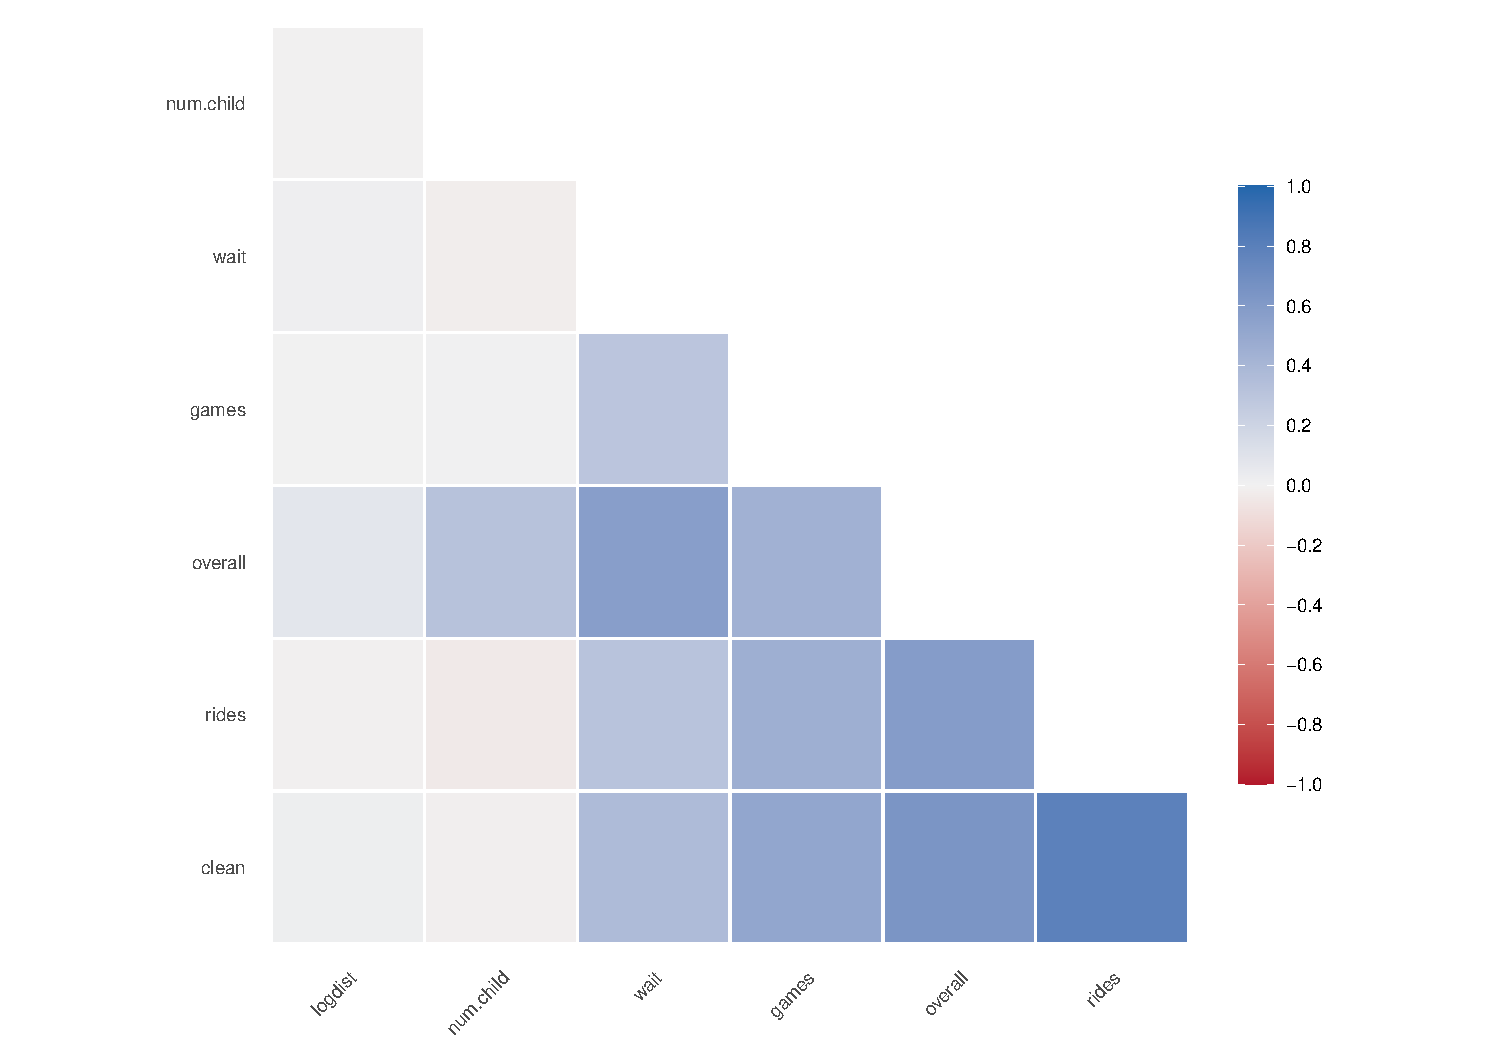
\includegraphics[width=0.5\textwidth,height=\textheight]{007_identifying_drivers_of_outcomes_linear_models_files/figure-beamer/unnamed-chunk-6-1.pdf}
\end{center}
\end{frame}

\begin{frame}[fragile]{}
\phantomsection\label{section-8}
\begin{itemize}
\tightlist
\item
  \textbf{Bivariate Association: the base R way}
\end{itemize}

\tiny

\begin{Shaded}
\begin{Highlighting}[]
\FunctionTok{plot}\NormalTok{(overall}\SpecialCharTok{\textasciitilde{}}\NormalTok{rides, }\AttributeTok{data=}\NormalTok{amusement\_park,}
     \AttributeTok{xlab=}\StringTok{"Satisfaction with Rides"}\NormalTok{, }\AttributeTok{ylab=}\StringTok{"Overall Satisfaction"}\NormalTok{)}
\FunctionTok{abline}\NormalTok{(}\AttributeTok{reg =} \FunctionTok{lm}\NormalTok{(}\AttributeTok{formula =}\NormalTok{ overall}\SpecialCharTok{\textasciitilde{}}\NormalTok{rides, }\AttributeTok{data =}\NormalTok{ amusement\_park), }
       \AttributeTok{col =} \StringTok{\textquotesingle{}blue\textquotesingle{}}\NormalTok{)}
\end{Highlighting}
\end{Shaded}

\begin{center}
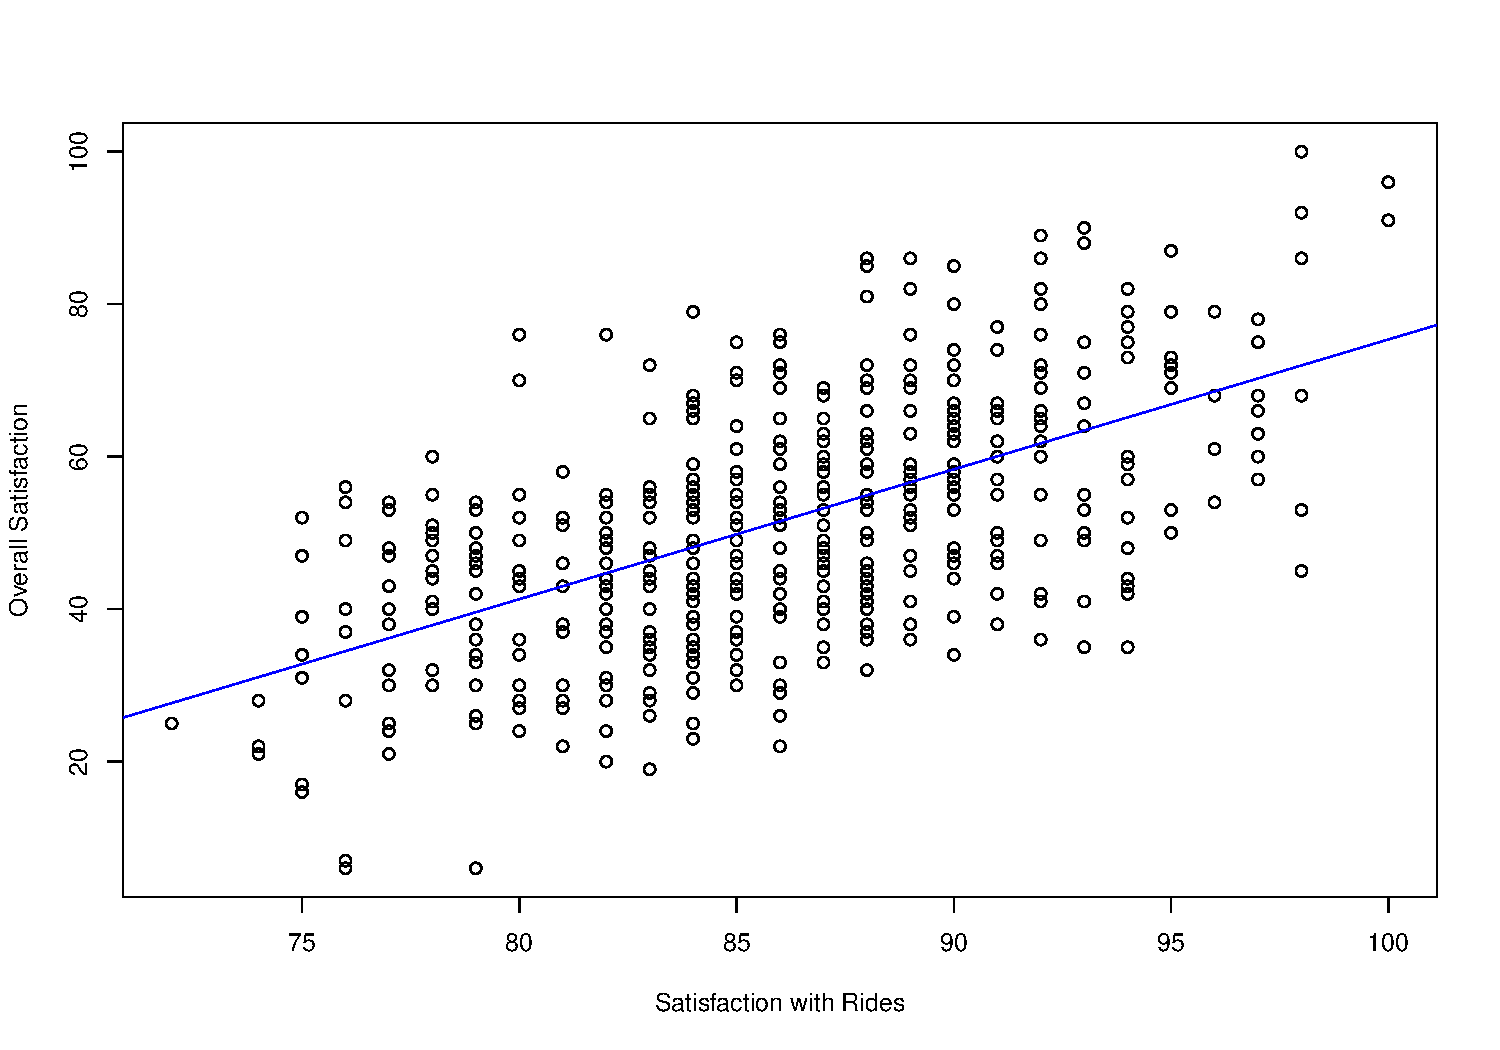
\includegraphics[width=0.5\textwidth,height=\textheight]{007_identifying_drivers_of_outcomes_linear_models_files/figure-beamer/unnamed-chunk-7-1.pdf}
\end{center}
\end{frame}

\begin{frame}[fragile]{}
\phantomsection\label{section-9}
\begin{itemize}
\tightlist
\item
  \textbf{Bivariate Association: the tidyverse way}
\end{itemize}

\tiny

\begin{Shaded}
\begin{Highlighting}[]
\NormalTok{amusement\_park }\SpecialCharTok{|\textgreater{}} \FunctionTok{ggplot}\NormalTok{(}\FunctionTok{aes}\NormalTok{(}\AttributeTok{x =}\NormalTok{ rides, }\AttributeTok{y =}\NormalTok{ overall)) }\SpecialCharTok{+}
  \FunctionTok{geom\_point}\NormalTok{() }\SpecialCharTok{+} 
  \FunctionTok{geom\_smooth}\NormalTok{(}\AttributeTok{method =} \StringTok{\textquotesingle{}lm\textquotesingle{}}\NormalTok{, }
              \AttributeTok{color =} \StringTok{\textquotesingle{}blue\textquotesingle{}}\NormalTok{, }
              \AttributeTok{se =} \ConstantTok{FALSE}\NormalTok{) }\SpecialCharTok{+} 
  \FunctionTok{labs}\NormalTok{(}\AttributeTok{x =} \StringTok{"Satisfaction with Rides"}\NormalTok{,}
       \AttributeTok{y =} \StringTok{"Overall Satisfaction"}\NormalTok{)}
\end{Highlighting}
\end{Shaded}

\begin{center}
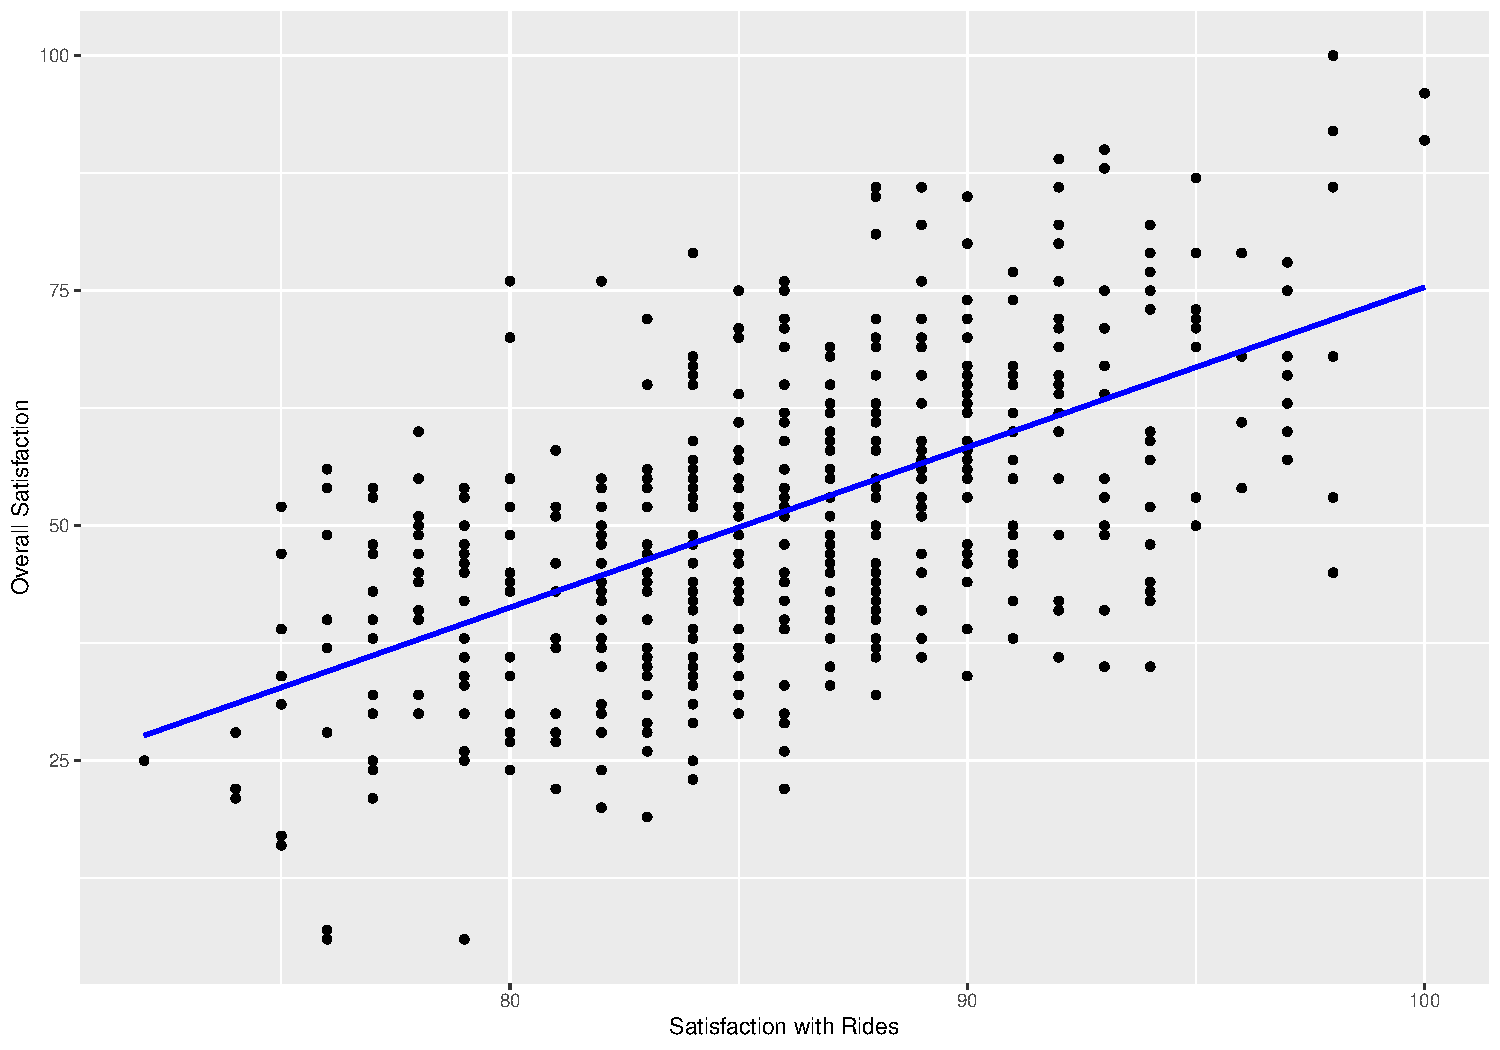
\includegraphics[width=0.5\textwidth,height=\textheight]{007_identifying_drivers_of_outcomes_linear_models_files/figure-beamer/unnamed-chunk-8-1.pdf}
\end{center}
\end{frame}

\begin{frame}{}
\phantomsection\label{section-10}
\begin{itemize}
\tightlist
\item
  Linear Model with a Single Predictor
\end{itemize}

\begin{center}
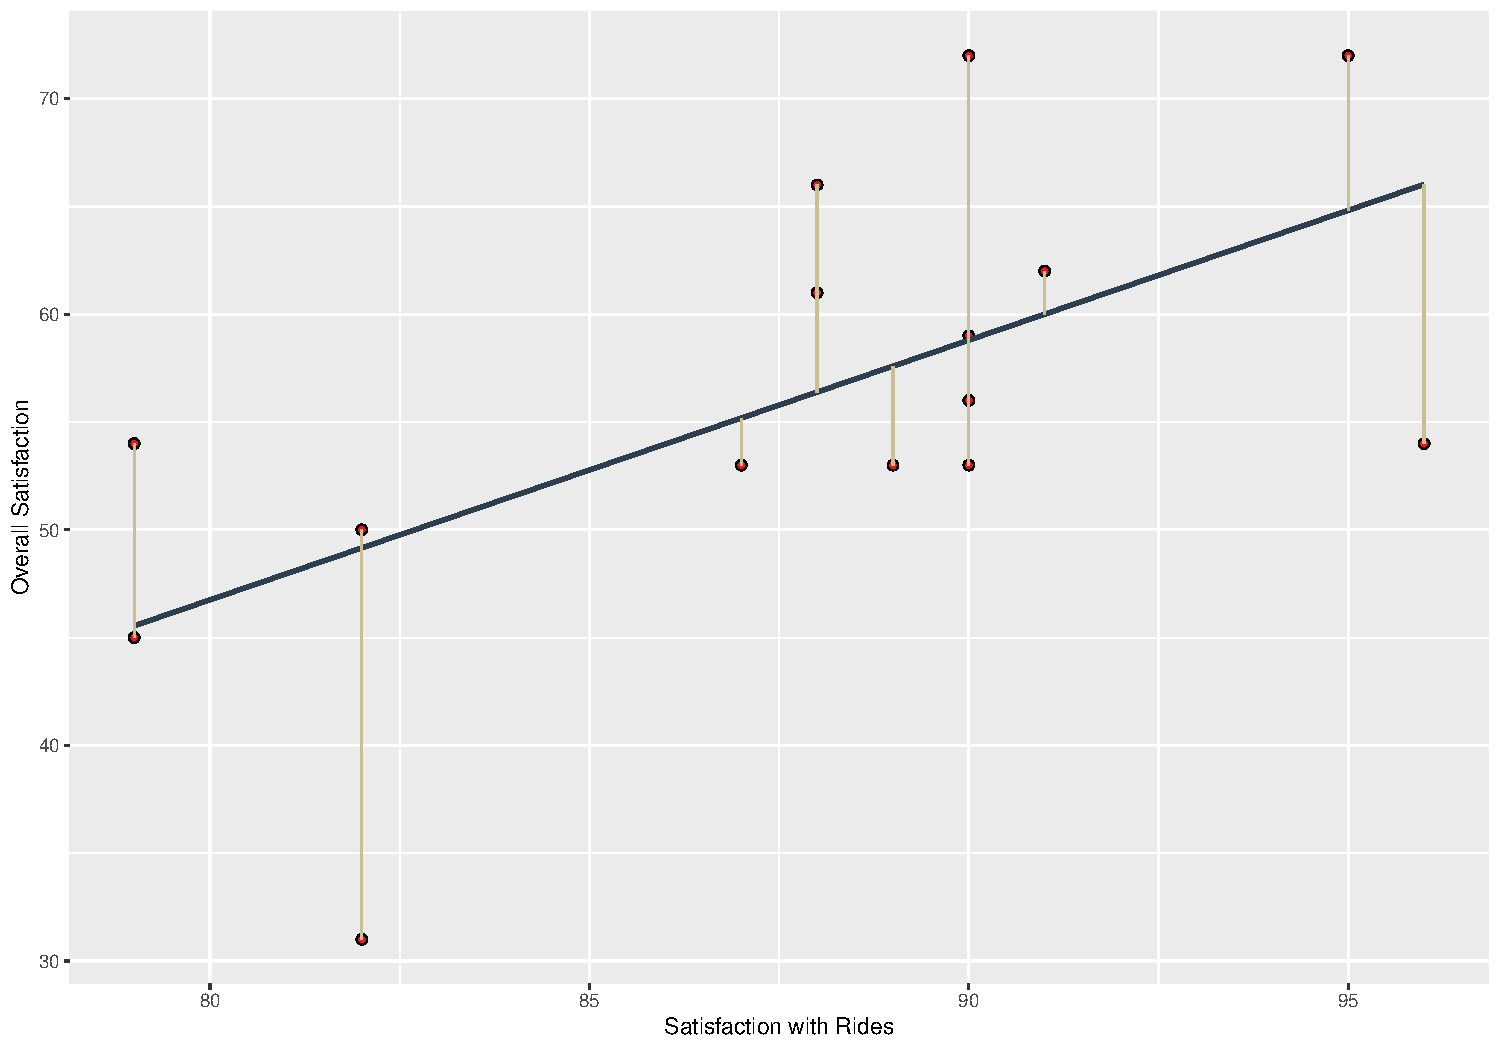
\includegraphics[width=0.8\textwidth,height=\textheight]{007_identifying_drivers_of_outcomes_linear_models_files/figure-beamer/unnamed-chunk-9-1.pdf}
\end{center}
\end{frame}

\begin{frame}[fragile]{}
\phantomsection\label{section-11}
\begin{itemize}
\tightlist
\item
  Linear Model with a Single Predictor
\end{itemize}

\[overall_{i} = \beta_0 + \beta_1 rides_i + \epsilon_i \text{ where } \epsilon_i \sim \mathcal{N}(0, \sigma^2) \text{ and } i = 1, \ldots, 500\]
\[\widehat{overall}_{i} = \widehat{\beta}_0 + \widehat{\beta}_1 rides_i \text{ and } \widehat{\sigma}^2 \text{ where } i = 1, \ldots, 500\]
\[overall_{i} - \widehat{overall}_{i} = \widehat{\epsilon}_i \text{ where } i = 1, \ldots, 500\]

\tiny

\begin{Shaded}
\begin{Highlighting}[]
\NormalTok{model1 }\OtherTok{\textless{}{-}} \FunctionTok{lm}\NormalTok{(}\AttributeTok{formula =}\NormalTok{ overall }\SpecialCharTok{\textasciitilde{}}\NormalTok{ rides, }\AttributeTok{data =}\NormalTok{ amusement\_park)}
\NormalTok{model1}
\end{Highlighting}
\end{Shaded}

\begin{verbatim}

Call:
lm(formula = overall ~ rides, data = amusement_park)

Coefficients:
(Intercept)        rides  
    -94.962        1.703  
\end{verbatim}
\end{frame}

\begin{frame}[fragile]{}
\phantomsection\label{section-12}
\begin{itemize}
\tightlist
\item
  Linear Model with a Single Predictor
\end{itemize}

\tiny

\begin{Shaded}
\begin{Highlighting}[]
\FunctionTok{ls.str}\NormalTok{(model1)}
\end{Highlighting}
\end{Shaded}

\begin{verbatim}
assign :  int [1:2] 0 1
call :  language lm(formula = overall ~ rides, data = amusement_park)
coefficients :  Named num [1:2] -95 1.7
df.residual :  int 498
effects :  Named num [1:500] -1146.2 -207.9 11.5 -17.9 20.3 ...
fitted.values :  Named num [1:500] 53.2 53.2 49.8 54.9 48.1 ...
model : 'data.frame':   500 obs. of  2 variables:
 $ overall: num  47 65 61 37 68 27 40 30 58 36 ...
 $ rides  : num  87 87 85 88 84 81 77 82 90 88 ...
qr : List of 5
 $ qr   : num [1:500, 1:2] -22.3607 0.0447 0.0447 0.0447 0.0447 ...
 $ qraux: num [1:2] 1.04 1.01
 $ pivot: int [1:2] 1 2
 $ tol  : num 1e-07
 $ rank : int 2
rank :  int 2
residuals :  Named num [1:500] -6.22 11.78 11.18 -17.93 19.89 ...
terms : Classes 'terms', 'formula'  language overall ~ rides
xlevels :  Named list()
\end{verbatim}
\end{frame}

\begin{frame}[fragile]{}
\phantomsection\label{section-13}
\begin{itemize}
\tightlist
\item
  Linear Model with a Single Predictor
\end{itemize}

\tiny

\begin{Shaded}
\begin{Highlighting}[]
\FunctionTok{summary}\NormalTok{(model1)}
\end{Highlighting}
\end{Shaded}

\begin{verbatim}

Call:
lm(formula = overall ~ rides, data = amusement_park)

Residuals:
    Min      1Q  Median      3Q     Max 
-33.597 -10.048   0.425   8.694  34.699 

Coefficients:
            Estimate Std. Error t value Pr(>|t|)    
(Intercept) -94.9622     9.0790  -10.46   <2e-16 ***
rides         1.7033     0.1055   16.14   <2e-16 ***
---
Signif. codes:  0 '***' 0.001 '**' 0.01 '*' 0.05 '.' 0.1 ' ' 1

Residual standard error: 12.88 on 498 degrees of freedom
Multiple R-squared:  0.3434,    Adjusted R-squared:  0.3421 
F-statistic: 260.4 on 1 and 498 DF,  p-value: < 2.2e-16
\end{verbatim}
\end{frame}

\begin{frame}[fragile]{}
\phantomsection\label{section-14}
\begin{itemize}
\tightlist
\item
  Linear Model with a Single Predictor
\end{itemize}

\tiny

\begin{Shaded}
\begin{Highlighting}[]
\NormalTok{model1}\SpecialCharTok{$}\NormalTok{coefficients}
\end{Highlighting}
\end{Shaded}

\begin{verbatim}
(Intercept)       rides 
 -94.962246    1.703285 
\end{verbatim}

\begin{Shaded}
\begin{Highlighting}[]
\CommentTok{\# Make some predictions}
\CommentTok{\# We want to forecast the overall satisfaction rating}
\CommentTok{\# if the satisfaction with rides is 95}
\SpecialCharTok{{-}}\FloatTok{94.962246} \SpecialCharTok{+} \FloatTok{1.703285}\SpecialCharTok{*}\DecValTok{95}
\end{Highlighting}
\end{Shaded}

\begin{verbatim}
[1] 66.84983
\end{verbatim}
\end{frame}

\begin{frame}[fragile]{}
\phantomsection\label{section-15}
\begin{itemize}
\item
  Linear Model with a Single Predictor

  \begin{itemize}
  \item
    Std. Error column

    \begin{itemize}
    \tightlist
    \item
      Indicates uncertainty in the coefficient estimate
    \item
      We can build a confidence interval
    \end{itemize}
  \end{itemize}
\end{itemize}

\tiny

\begin{Shaded}
\begin{Highlighting}[]
\FunctionTok{summary}\NormalTok{(model1)}\SpecialCharTok{$}\NormalTok{coefficients[, }\DecValTok{2}\NormalTok{]}
\end{Highlighting}
\end{Shaded}

\begin{verbatim}
(Intercept)       rides 
  9.0790049   0.1055462 
\end{verbatim}

\begin{Shaded}
\begin{Highlighting}[]
\FunctionTok{confint}\NormalTok{(model1, }\AttributeTok{level =} \FloatTok{0.95}\NormalTok{)}
\end{Highlighting}
\end{Shaded}

\begin{verbatim}
                  2.5 %     97.5 %
(Intercept) -112.800120 -77.124371
rides          1.495915   1.910656
\end{verbatim}
\end{frame}

\begin{frame}[fragile]{}
\phantomsection\label{section-16}
\begin{itemize}
\tightlist
\item
  Linear Model with a Single Predictor
\end{itemize}

\tiny

\begin{Shaded}
\begin{Highlighting}[]
\FunctionTok{par}\NormalTok{(}\AttributeTok{mfrow=}\FunctionTok{c}\NormalTok{(}\DecValTok{2}\NormalTok{,}\DecValTok{2}\NormalTok{))}
\FunctionTok{plot}\NormalTok{(model1)}
\end{Highlighting}
\end{Shaded}

\begin{center}
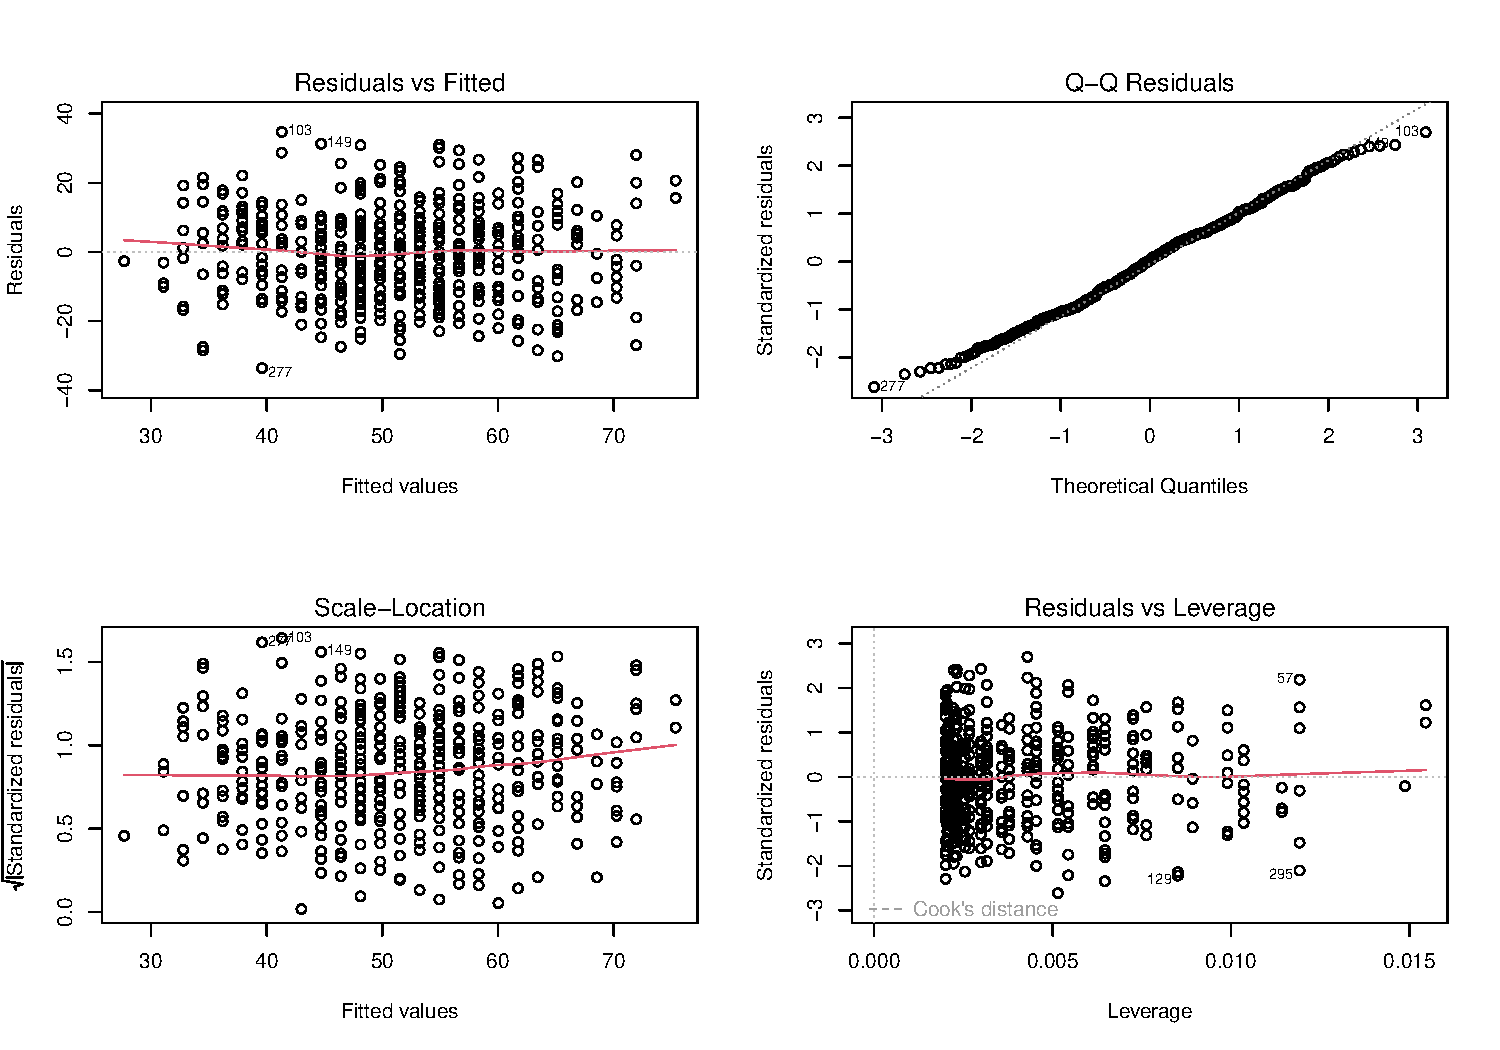
\includegraphics[width=0.5\textwidth,height=\textheight]{007_identifying_drivers_of_outcomes_linear_models_files/figure-beamer/unnamed-chunk-15-1.pdf}
\end{center}

\begin{Shaded}
\begin{Highlighting}[]
\FunctionTok{par}\NormalTok{(}\AttributeTok{mfrow=}\FunctionTok{c}\NormalTok{(}\DecValTok{1}\NormalTok{,}\DecValTok{1}\NormalTok{))}
\end{Highlighting}
\end{Shaded}
\end{frame}

\begin{frame}{}
\phantomsection\label{section-17}
\begin{itemize}
\item
  Linear Model with a Single Predictor

  \begin{itemize}
  \item
    \textbf{Linearity}: plot \((1,1)\)

    \begin{itemize}
    \tightlist
    \item
      Reference line should be flat and horizontal
    \end{itemize}
  \item
    \textbf{Normality of residuals}: plot \((1,2)\)

    \begin{itemize}
    \tightlist
    \item
      Dots should fall along the line
    \end{itemize}
  \item
    \textbf{Homogeneity of variance}: plot \((2,1)\)

    \begin{itemize}
    \tightlist
    \item
      Reference line should be flat and horizontal
    \end{itemize}
  \item
    \textbf{Influential observations}: plot \((2,2)\)

    \begin{itemize}
    \tightlist
    \item
      Points should be inside the contour lines
    \end{itemize}
  \end{itemize}
\end{itemize}
\end{frame}

\begin{frame}[fragile]{}
\phantomsection\label{section-18}
\begin{itemize}
\tightlist
\item
  Linear Model with Multiple Predictors
\end{itemize}

\[\begin{split}
   overall_{i} & = \beta_0 + \beta_1 rides_i + \beta_2 games_i \\
   & + \beta_3 wait_i + \beta_4 clean_i + \epsilon_i \\
   & \text{ where } \epsilon_i \sim \mathcal{N}(0, \sigma^2) \text{ and } i = 1, \ldots, 500
   \end{split}\]

\tiny

\begin{Shaded}
\begin{Highlighting}[]
\NormalTok{model2 }\OtherTok{\textless{}{-}} \FunctionTok{lm}\NormalTok{(}\AttributeTok{formula =}\NormalTok{ overall }\SpecialCharTok{\textasciitilde{}}\NormalTok{ rides }\SpecialCharTok{+}\NormalTok{ games }\SpecialCharTok{+}\NormalTok{ wait }\SpecialCharTok{+}\NormalTok{ clean, }
             \AttributeTok{data =}\NormalTok{ amusement\_park)}
\NormalTok{model2}
\end{Highlighting}
\end{Shaded}

\begin{verbatim}

Call:
lm(formula = overall ~ rides + games + wait + clean, data = amusement_park)

Coefficients:
(Intercept)        rides        games         wait        clean  
  -131.4092       0.5291       0.1533       0.5533       0.9842  
\end{verbatim}
\end{frame}

\begin{frame}[fragile]{}
\phantomsection\label{section-19}
\begin{itemize}
\tightlist
\item
  Linear Model with Multiple Predictors
\end{itemize}

\tiny

\begin{Shaded}
\begin{Highlighting}[]
\FunctionTok{par}\NormalTok{(}\AttributeTok{mfrow=}\FunctionTok{c}\NormalTok{(}\DecValTok{2}\NormalTok{,}\DecValTok{2}\NormalTok{))}
\FunctionTok{plot}\NormalTok{(model2)}
\end{Highlighting}
\end{Shaded}

\begin{center}
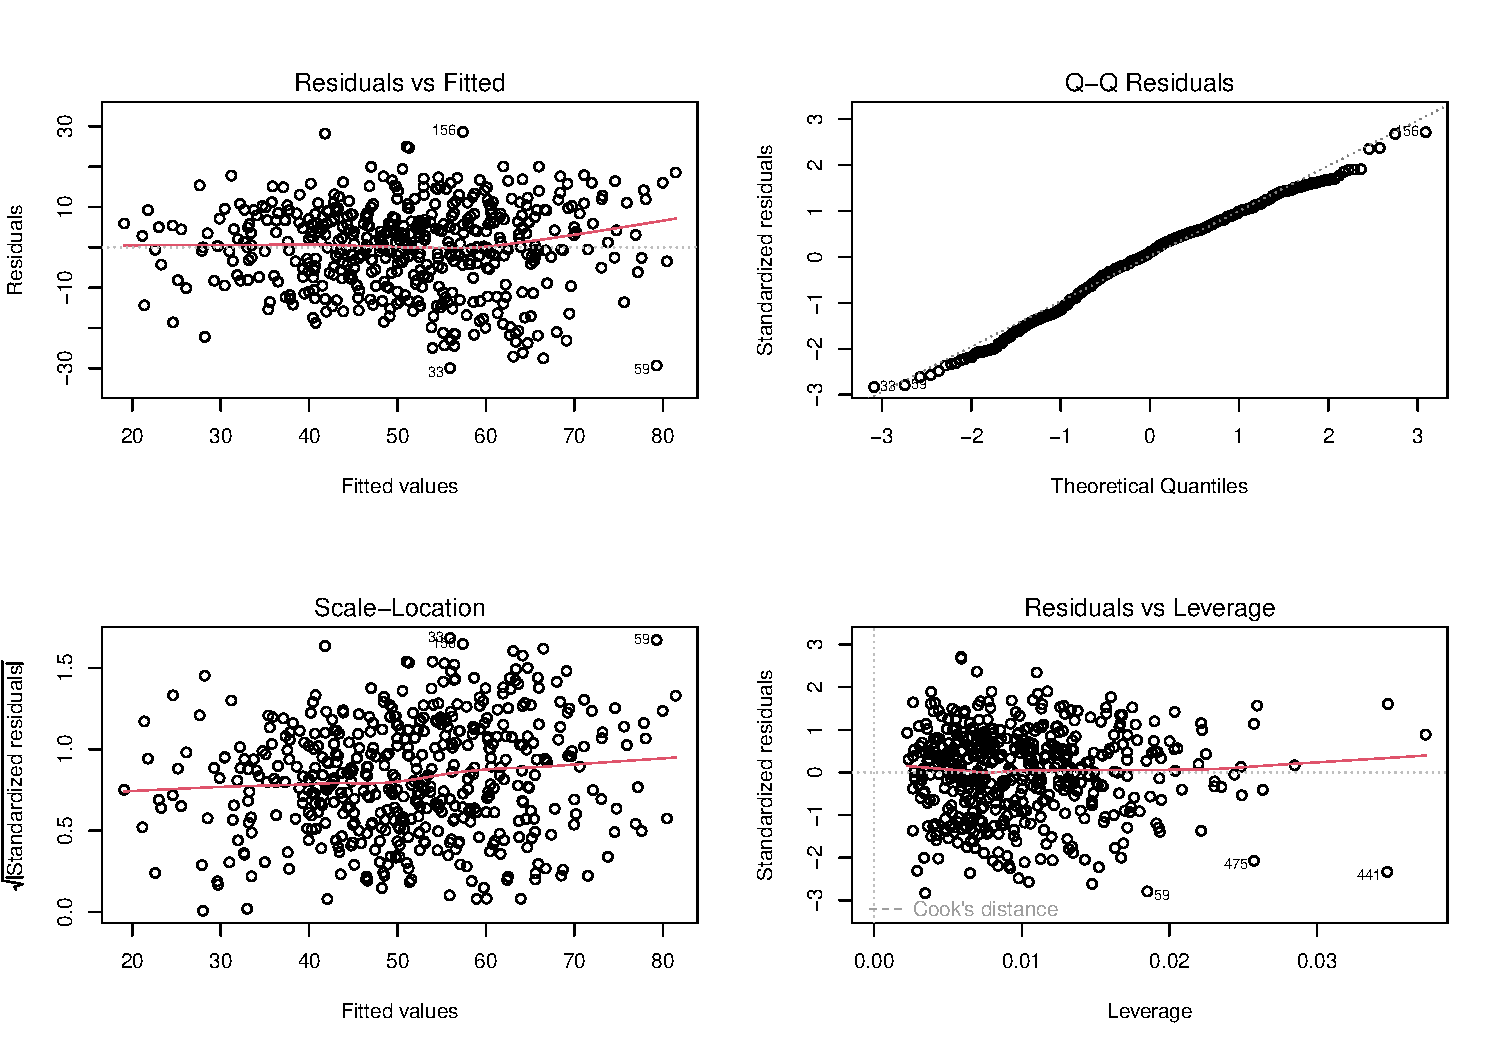
\includegraphics[width=0.5\textwidth,height=\textheight]{007_identifying_drivers_of_outcomes_linear_models_files/figure-beamer/unnamed-chunk-17-1.pdf}
\end{center}

\begin{Shaded}
\begin{Highlighting}[]
\FunctionTok{par}\NormalTok{(}\AttributeTok{mfrow=}\FunctionTok{c}\NormalTok{(}\DecValTok{1}\NormalTok{,}\DecValTok{1}\NormalTok{))}
\end{Highlighting}
\end{Shaded}
\end{frame}

\begin{frame}[fragile]{}
\phantomsection\label{section-20}
\begin{itemize}
\tightlist
\item
  Linear Model with Multiple Predictors
\end{itemize}

\tiny

\begin{Shaded}
\begin{Highlighting}[]
\FunctionTok{summary}\NormalTok{(model2)}
\end{Highlighting}
\end{Shaded}

\begin{verbatim}

Call:
lm(formula = overall ~ rides + games + wait + clean, data = amusement_park)

Residuals:
    Min      1Q  Median      3Q     Max 
-29.944  -6.841   1.072   7.167  28.618 

Coefficients:
              Estimate Std. Error t value Pr(>|t|)    
(Intercept) -131.40919    8.33377 -15.768  < 2e-16 ***
rides          0.52908    0.14207   3.724 0.000219 ***
games          0.15334    0.06908   2.220 0.026903 *  
wait           0.55333    0.04781  11.573  < 2e-16 ***
clean          0.98421    0.15987   6.156 1.54e-09 ***
---
Signif. codes:  0 '***' 0.001 '**' 0.01 '*' 0.05 '.' 0.1 ' ' 1

Residual standard error: 10.59 on 495 degrees of freedom
Multiple R-squared:  0.5586,    Adjusted R-squared:  0.5551 
F-statistic: 156.6 on 4 and 495 DF,  p-value: < 2.2e-16
\end{verbatim}
\end{frame}

\begin{frame}[fragile]{}
\phantomsection\label{section-21}
\begin{itemize}
\tightlist
\item
  Linear Model with Multiple Predictors
\end{itemize}

\(H_0: \beta_1 = 0\)

\(H_1: \beta_1 \neq 0\)

\(t_{rides} = \frac{\hat{\beta}_1 - \beta_1}{\sqrt{\widehat{Var(\hat{\beta}_1)}}} = \frac{0.529078 - 0}{0.14207176} = 3.724019\)

\tiny

\begin{Shaded}
\begin{Highlighting}[]
\NormalTok{model2}\SpecialCharTok{$}\NormalTok{coefficients}
\end{Highlighting}
\end{Shaded}

\begin{verbatim}
 (Intercept)        rides        games         wait        clean 
-131.4091939    0.5290780    0.1533361    0.5533264    0.9842126 
\end{verbatim}

\begin{Shaded}
\begin{Highlighting}[]
\CommentTok{\# Calculate the variance{-}covariance matrix, extract}
\CommentTok{\# the diagonal and calculate the standard deviaton of}
\CommentTok{\# the parameters}
\NormalTok{model2 }\SpecialCharTok{|\textgreater{}} \FunctionTok{vcov}\NormalTok{() }\SpecialCharTok{|\textgreater{}} \FunctionTok{diag}\NormalTok{() }\SpecialCharTok{|\textgreater{}} \FunctionTok{sqrt}\NormalTok{()}
\end{Highlighting}
\end{Shaded}

\begin{verbatim}
(Intercept)       rides       games        wait       clean 
 8.33376643  0.14207176  0.06908486  0.04781282  0.15986712 
\end{verbatim}
\end{frame}

\begin{frame}{}
\phantomsection\label{section-22}
\begin{itemize}
\tightlist
\item
  Linear Model with Multiple Predictors
\end{itemize}

\begin{center}
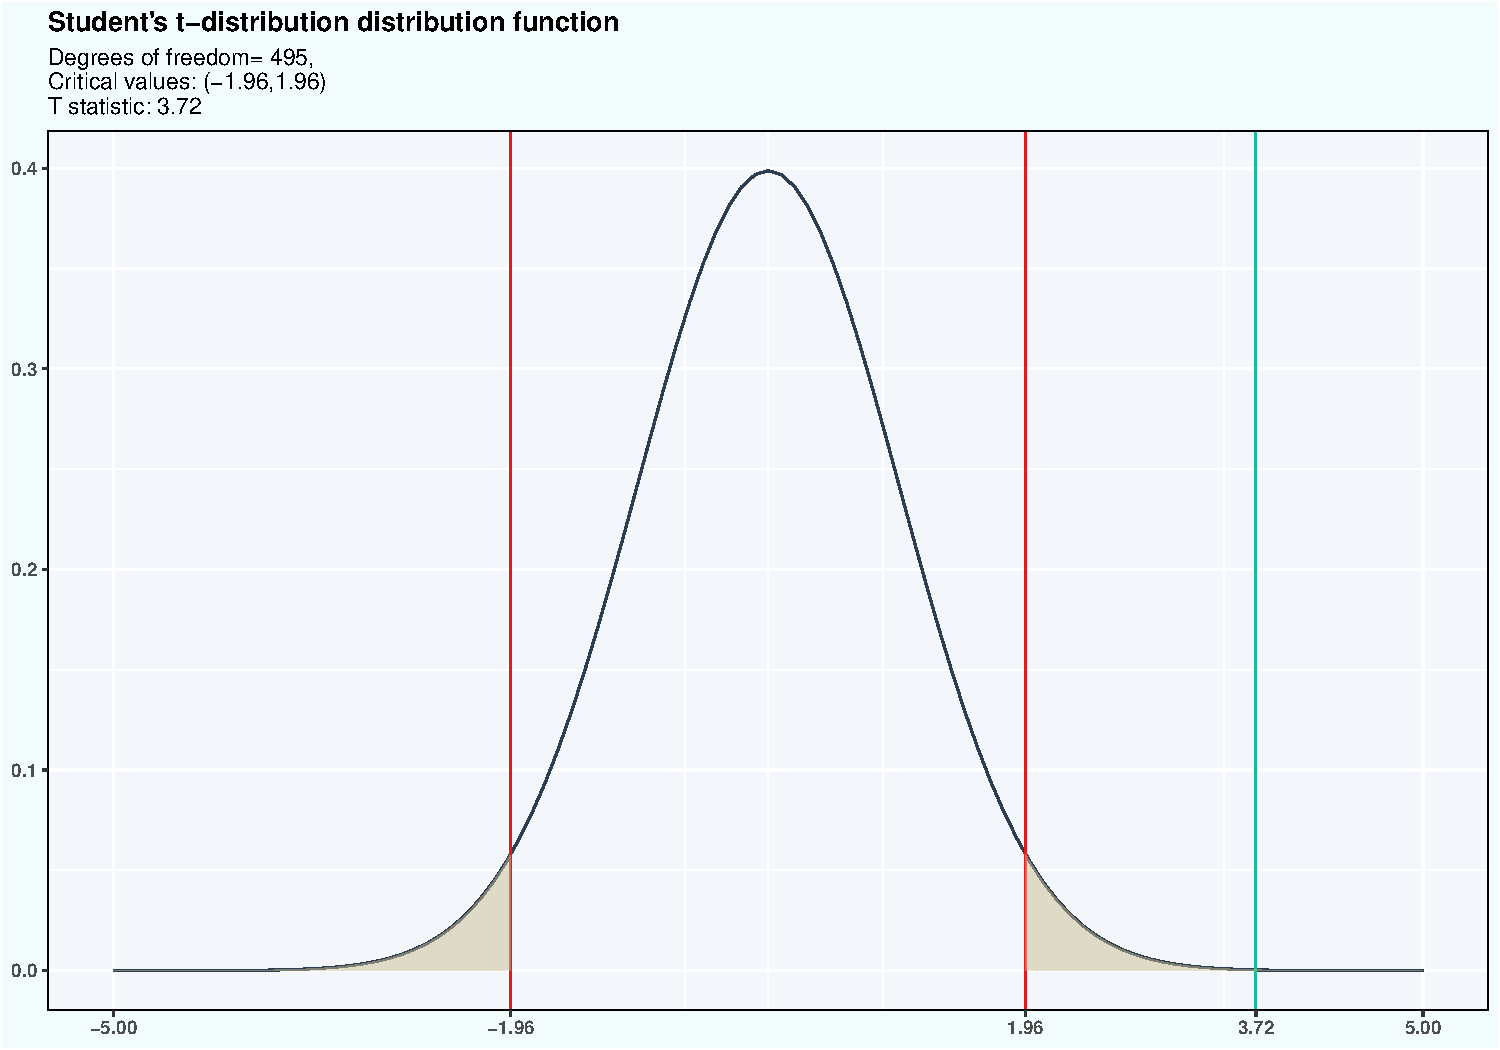
\includegraphics[width=0.8\textwidth,height=\textheight]{007_identifying_drivers_of_outcomes_linear_models_files/figure-beamer/unnamed-chunk-20-1.pdf}
\end{center}
\end{frame}

\begin{frame}[fragile]{}
\phantomsection\label{section-23}
\begin{itemize}
\tightlist
\item
  Linear Model with Multiple Predictors
\end{itemize}

\tiny

\begin{Shaded}
\begin{Highlighting}[]
\FunctionTok{confint}\NormalTok{(model2, }\AttributeTok{level =} \FloatTok{0.95}\NormalTok{)}
\end{Highlighting}
\end{Shaded}

\begin{verbatim}
                    2.5 %       97.5 %
(Intercept) -147.78311147 -115.0352764
rides          0.24993998    0.8082161
games          0.01760038    0.2890718
wait           0.45938535    0.6472675
clean          0.67011082    1.2983144
\end{verbatim}
\end{frame}

\begin{frame}[fragile]{}
\phantomsection\label{section-24}
\begin{itemize}
\tightlist
\item
  Linear Model with Multiple Predictors
\end{itemize}

\tiny

\begin{Shaded}
\begin{Highlighting}[]
\FunctionTok{library}\NormalTok{(coefplot) }\CommentTok{\# Remember to install the package if it is not installed}
\FunctionTok{coefplot}\NormalTok{(}\AttributeTok{model =}\NormalTok{ model2, }
         \CommentTok{\# The intercept is relatively large: {-}131.4092 }
         \AttributeTok{intercept =} \ConstantTok{FALSE}\NormalTok{,}
         \AttributeTok{ylab=}\StringTok{"Rating of Feature"}\NormalTok{, }
         \AttributeTok{xlab=}\StringTok{"Association with Overall Satisfaction"}\NormalTok{,}
         \AttributeTok{lwdOuter =} \FloatTok{1.5}\NormalTok{)}
\end{Highlighting}
\end{Shaded}

\begin{center}
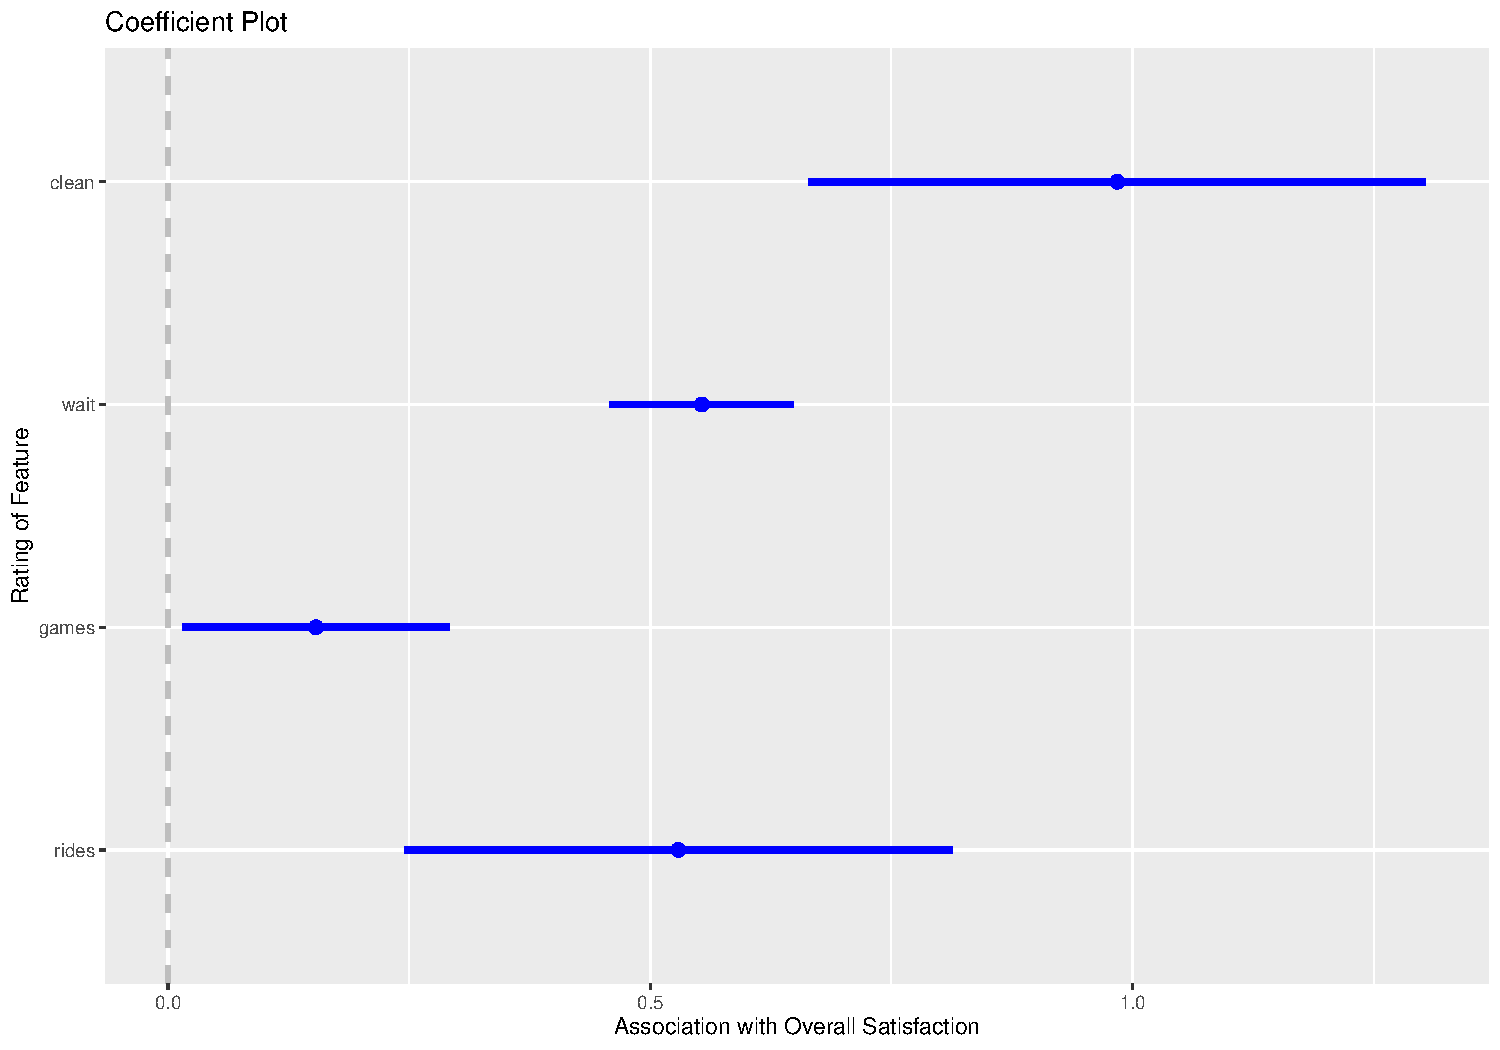
\includegraphics[width=0.5\textwidth,height=\textheight]{007_identifying_drivers_of_outcomes_linear_models_files/figure-beamer/unnamed-chunk-22-1.pdf}
\end{center}
\end{frame}

\begin{frame}[fragile]{}
\phantomsection\label{section-25}
\begin{itemize}
\tightlist
\item
  Comparing models
\end{itemize}

\tiny

\begin{Shaded}
\begin{Highlighting}[]
\FunctionTok{summary}\NormalTok{(model1)}\SpecialCharTok{$}\NormalTok{r.squared}
\end{Highlighting}
\end{Shaded}

\begin{verbatim}
[1] 0.3433799
\end{verbatim}

\begin{Shaded}
\begin{Highlighting}[]
\FunctionTok{summary}\NormalTok{(model2)}\SpecialCharTok{$}\NormalTok{r.squared}
\end{Highlighting}
\end{Shaded}

\begin{verbatim}
[1] 0.558621
\end{verbatim}

\begin{Shaded}
\begin{Highlighting}[]
\FunctionTok{summary}\NormalTok{(model1)}\SpecialCharTok{$}\NormalTok{adj.r.squared}
\end{Highlighting}
\end{Shaded}

\begin{verbatim}
[1] 0.3420614
\end{verbatim}

\begin{Shaded}
\begin{Highlighting}[]
\FunctionTok{summary}\NormalTok{(model2)}\SpecialCharTok{$}\NormalTok{adj.r.squared}
\end{Highlighting}
\end{Shaded}

\begin{verbatim}
[1] 0.5550543
\end{verbatim}
\end{frame}

\begin{frame}[fragile]{}
\phantomsection\label{section-26}
\begin{itemize}
\item
  Comparing models

  \begin{itemize}
  \tightlist
  \item
    \textbf{Base R way}
  \end{itemize}
\end{itemize}

\tiny

\begin{Shaded}
\begin{Highlighting}[]
\FunctionTok{plot}\NormalTok{(}\AttributeTok{x =}\NormalTok{ amusement\_park}\SpecialCharTok{$}\NormalTok{overall, }\AttributeTok{y =} \FunctionTok{fitted}\NormalTok{(model1),}
     \AttributeTok{col =} \StringTok{"red"}\NormalTok{, }\AttributeTok{xlim =} \FunctionTok{c}\NormalTok{(}\DecValTok{0}\NormalTok{,}\DecValTok{100}\NormalTok{), }\AttributeTok{ylim =} \FunctionTok{c}\NormalTok{(}\DecValTok{0}\NormalTok{,}\DecValTok{100}\NormalTok{),}
     \AttributeTok{xlab =} \StringTok{"Actual Overall Satisfaction"}\NormalTok{, }
     \AttributeTok{ylab =} \StringTok{"Fitted Overall Satisfaction"}\NormalTok{)}
\FunctionTok{points}\NormalTok{(}\AttributeTok{x =}\NormalTok{ amusement\_park}\SpecialCharTok{$}\NormalTok{overall, }\AttributeTok{y =} \FunctionTok{fitted}\NormalTok{(model2),}
       \AttributeTok{col =} \StringTok{"blue"}\NormalTok{)}
\FunctionTok{legend}\NormalTok{(}\AttributeTok{x =} \StringTok{"topleft"}\NormalTok{, }\AttributeTok{legend =} \FunctionTok{c}\NormalTok{(}\StringTok{"Model 1"}\NormalTok{, }\StringTok{"Model 2"}\NormalTok{), }\AttributeTok{col =} \FunctionTok{c}\NormalTok{(}\StringTok{"red"}\NormalTok{, }\StringTok{"blue"}\NormalTok{), }\AttributeTok{pch =} \DecValTok{1}\NormalTok{)}
\end{Highlighting}
\end{Shaded}

\begin{center}
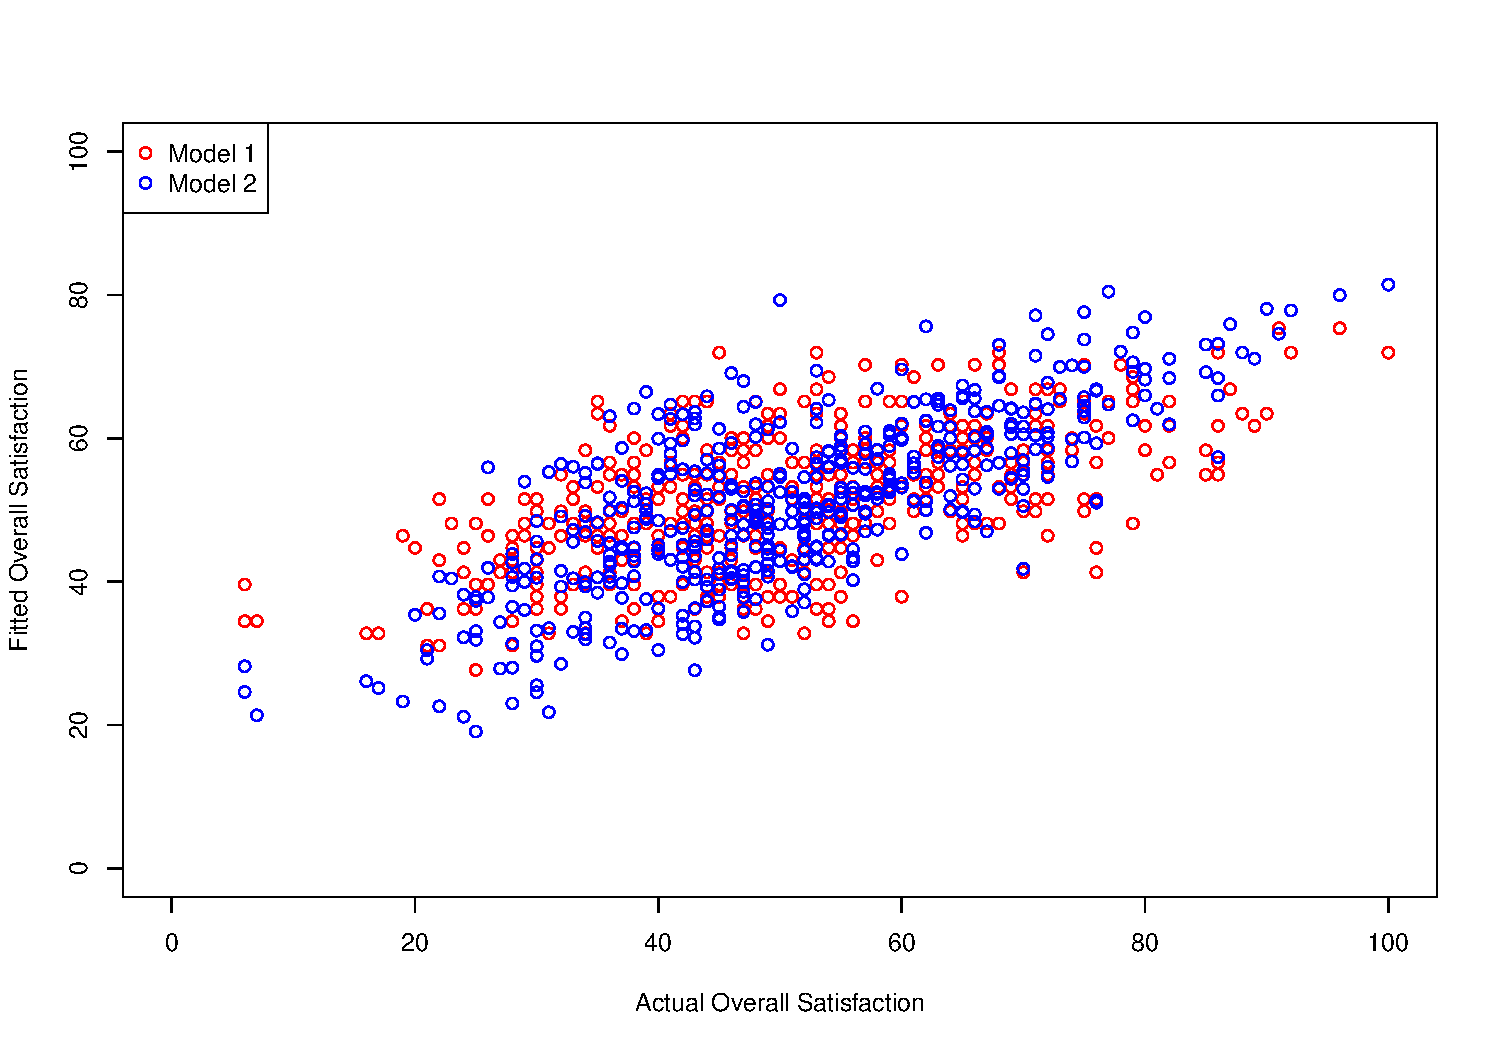
\includegraphics[width=0.5\textwidth,height=\textheight]{007_identifying_drivers_of_outcomes_linear_models_files/figure-beamer/unnamed-chunk-24-1.pdf}
\end{center}
\end{frame}

\begin{frame}[fragile]{}
\phantomsection\label{section-27}
\begin{itemize}
\item
  Comparing models

  \begin{itemize}
  \tightlist
  \item
    \textbf{Tidymodels and tidyverse way}: Prepare data
  \end{itemize}
\end{itemize}

\tiny

\begin{Shaded}
\begin{Highlighting}[]
\NormalTok{model1\_augment }\OtherTok{\textless{}{-}} \FunctionTok{augment}\NormalTok{(}\AttributeTok{x =}\NormalTok{ model1) }\SpecialCharTok{|\textgreater{}} \FunctionTok{mutate}\NormalTok{(}\AttributeTok{model =} \StringTok{"Model 1"}\NormalTok{)}
\NormalTok{model2\_augment }\OtherTok{\textless{}{-}} \FunctionTok{augment}\NormalTok{(}\AttributeTok{x =}\NormalTok{ model2) }\SpecialCharTok{|\textgreater{}} \FunctionTok{mutate}\NormalTok{(}\AttributeTok{model =} \StringTok{"Model 2"}\NormalTok{)}
\NormalTok{models\_performance }\OtherTok{\textless{}{-}}\NormalTok{ model1\_augment }\SpecialCharTok{|\textgreater{}} \FunctionTok{bind\_rows}\NormalTok{(model2\_augment)}

\NormalTok{models\_performance }\SpecialCharTok{|\textgreater{}} \FunctionTok{glimpse}\NormalTok{()}
\end{Highlighting}
\end{Shaded}

\begin{verbatim}
Rows: 1,000
Columns: 12
$ overall    <dbl> 47, 65, 61, 37, 68, 27, 40, 30, 58, 36, 71, 48, 75, 46, 59,~
$ rides      <dbl> 87, 87, 85, 88, 84, 81, 77, 82, 90, 88, 93, 79, 94, 81, 86,~
$ .fitted    <dbl> 53.22359, 53.22359, 49.81702, 54.92688, 48.11373, 43.00388,~
$ .resid     <dbl> -6.2235914, 11.7764086, 11.1829795, -17.9268769, 19.8862650~
$ .hat       <dbl> 0.002089430, 0.002089430, 0.002048063, 0.002311576, 0.00222~
$ .sigma     <dbl> 12.88964, 12.88182, 12.88289, 12.86751, 12.86171, 12.87260,~
$ .cooksd    <dbl> 2.449537e-04, 8.770564e-04, 7.751689e-04, 2.249493e-03, 2.6~
$ .std.resid <dbl> -0.48371422, 0.91529407, 0.86915315, -1.39348008, 1.5457218~
$ model      <chr> "Model 1", "Model 1", "Model 1", "Model 1", "Model 1", "Mod~
$ games      <dbl> NA, NA, NA, NA, NA, NA, NA, NA, NA, NA, NA, NA, NA, NA, NA,~
$ wait       <dbl> NA, NA, NA, NA, NA, NA, NA, NA, NA, NA, NA, NA, NA, NA, NA,~
$ clean      <dbl> NA, NA, NA, NA, NA, NA, NA, NA, NA, NA, NA, NA, NA, NA, NA,~
\end{verbatim}
\end{frame}

\begin{frame}[fragile]{}
\phantomsection\label{section-28}
\begin{itemize}
\item
  Comparing models

  \begin{itemize}
  \tightlist
  \item
    \textbf{Tidymodels and tidyverse way}: Visualize
  \end{itemize}
\end{itemize}

\tiny

\begin{Shaded}
\begin{Highlighting}[]
\NormalTok{models\_performance }\SpecialCharTok{|\textgreater{}} 
  \FunctionTok{ggplot}\NormalTok{() }\SpecialCharTok{+}
  \FunctionTok{geom\_point}\NormalTok{(}\FunctionTok{aes}\NormalTok{(}\AttributeTok{x =}\NormalTok{ overall, }\AttributeTok{y =}\NormalTok{ .fitted,}
                 \AttributeTok{color =}\NormalTok{ model)) }\SpecialCharTok{+}
  \FunctionTok{labs}\NormalTok{(}\AttributeTok{x =} \StringTok{"Actual Overall Satisfaction"}\NormalTok{,}
       \AttributeTok{y =} \StringTok{"Fitted Overall Satisfaction"}\NormalTok{)}
\end{Highlighting}
\end{Shaded}

\begin{center}
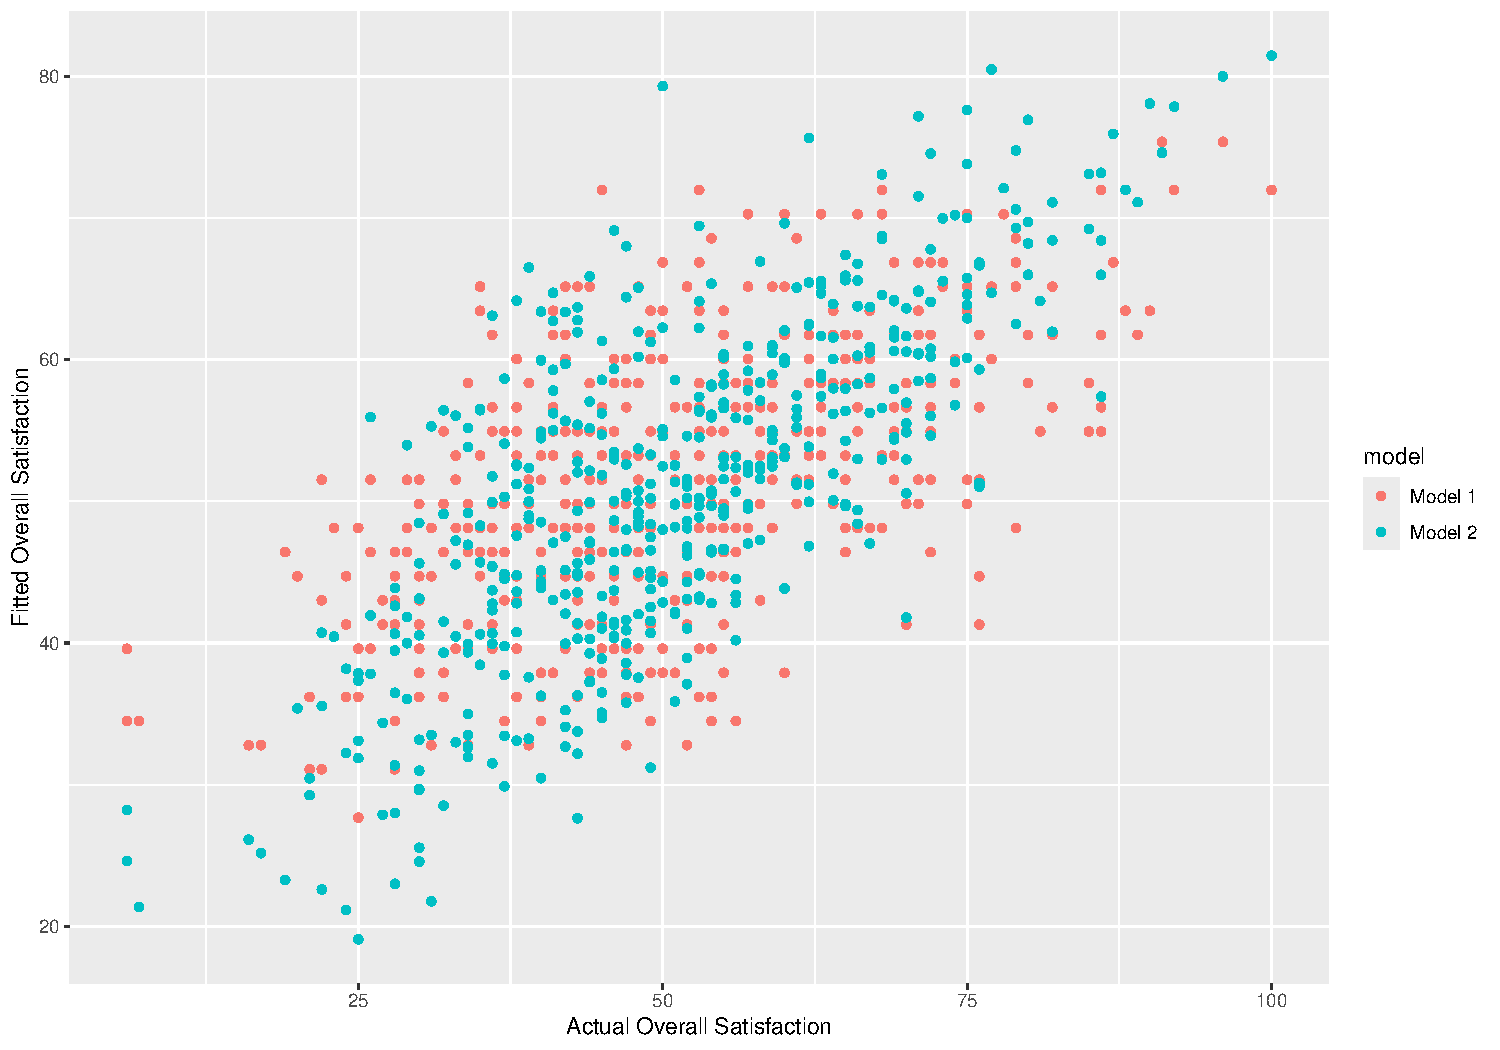
\includegraphics[width=0.5\textwidth,height=\textheight]{007_identifying_drivers_of_outcomes_linear_models_files/figure-beamer/unnamed-chunk-26-1.pdf}
\end{center}
\end{frame}

\begin{frame}[fragile]{}
\phantomsection\label{section-29}
\begin{itemize}
\item
  Comparing models

  \begin{itemize}
  \tightlist
  \item
    Analysis of variance (\texttt{anova}) for nested
    models\footnote<.->{This statistical analysis only make sense for
      nested models that are fitted with the same data where the
      convention is to include the models from smallest to largest. See
      \texttt{?anova.lm}}
  \end{itemize}
\end{itemize}

\tiny

\begin{Shaded}
\begin{Highlighting}[]
\NormalTok{anova\_lm }\OtherTok{\textless{}{-}} \FunctionTok{anova}\NormalTok{(model1, model2, }\AttributeTok{test =} \StringTok{"F"}\NormalTok{)}
\NormalTok{anova\_lm}
\end{Highlighting}
\end{Shaded}

\begin{verbatim}
Analysis of Variance Table

Model 1: overall ~ rides
Model 2: overall ~ rides + games + wait + clean
  Res.Df   RSS Df Sum of Sq      F    Pr(>F)    
1    498 82612                                  
2    495 55532  3     27080 80.463 < 2.2e-16 ***
---
Signif. codes:  0 '***' 0.001 '**' 0.01 '*' 0.05 '.' 0.1 ' ' 1
\end{verbatim}
\end{frame}

\begin{frame}{}
\phantomsection\label{section-30}
\begin{itemize}
\tightlist
\item
  Comparing models
\end{itemize}

\tiny

\(H_0: \beta_0 = \beta_1 = \beta_2 = \beta_3 = \beta_4 = 0\)

\(H_1: \text{At least one } \beta_j \neq 0 \text{ for } j = 0, 1, 2, 3, 4\)

\(F = \frac{\frac{RSS_1 - RSS_2}{p_2 - p_1}}{\frac{RSS_2}{n - p_2}} = \frac{\frac{82611.81 - 55531.53}{5 - 2}}{\frac{55531.53}{500 - 5}} = 80.46323\)

\begin{center}
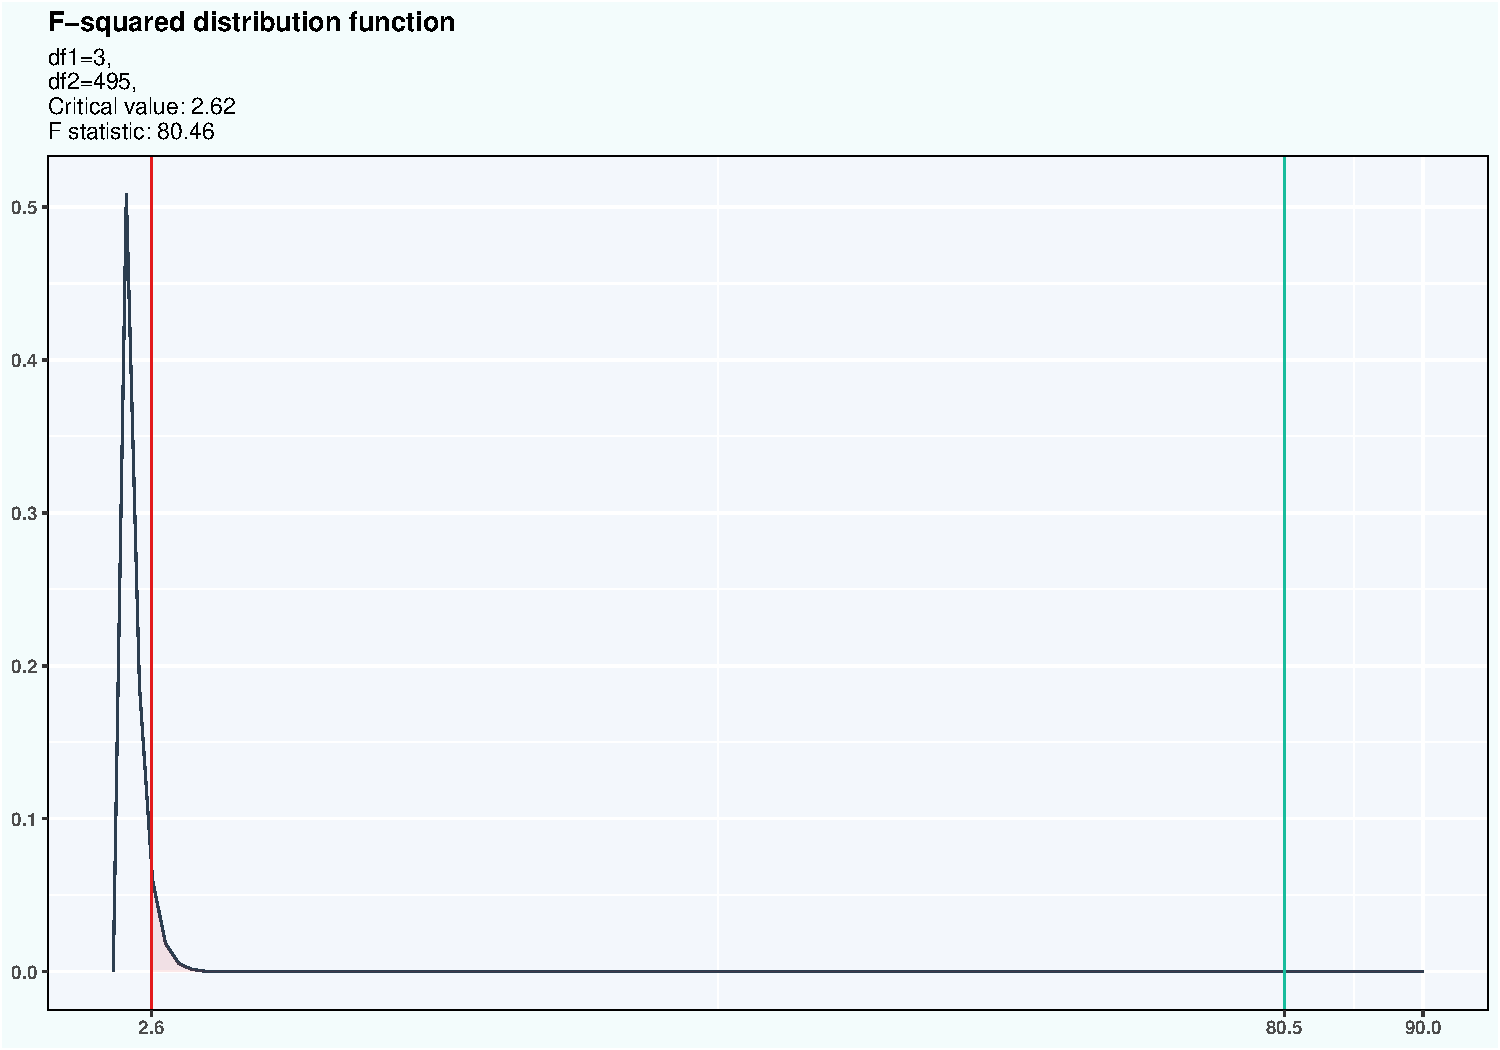
\includegraphics[width=0.5\textwidth,height=\textheight]{007_identifying_drivers_of_outcomes_linear_models_files/figure-beamer/unnamed-chunk-28-1.pdf}
\end{center}
\end{frame}

\begin{frame}[fragile]{}
\phantomsection\label{section-31}
\begin{itemize}
\tightlist
\item
  Predictions
\end{itemize}

\[\begin{split}
   \widehat{overall}_{j} & = \widehat{\beta}_0 + \widehat{\beta}_1 rides_j + \widehat{\beta}_2 games_j \\
   & + \widehat{\beta}_3 wait_j + \widehat{\beta}_4 clean_j
   \end{split}\]

\tiny

\begin{Shaded}
\begin{Highlighting}[]
\FunctionTok{coef}\NormalTok{(model2) }\SpecialCharTok{|\textgreater{}} \FunctionTok{enframe}\NormalTok{(}\AttributeTok{name =} \StringTok{"coef"}\NormalTok{)}
\end{Highlighting}
\end{Shaded}

\begin{verbatim}
# A tibble: 5 x 2
  coef           value
  <chr>          <dbl>
1 (Intercept) -131.   
2 rides          0.529
3 games          0.153
4 wait           0.553
5 clean          0.984
\end{verbatim}
\end{frame}

\begin{frame}[fragile]{}
\phantomsection\label{section-32}
\begin{itemize}
\item
  Predictions

  \begin{itemize}
  \tightlist
  \item
    Manual
  \end{itemize}
\end{itemize}

\tiny

\begin{Shaded}
\begin{Highlighting}[]
\NormalTok{(}\FunctionTok{coef}\NormalTok{(model2)[}\StringTok{"(Intercept)"}\NormalTok{]}\SpecialCharTok{*}\DecValTok{1} \SpecialCharTok{+} \FunctionTok{coef}\NormalTok{(model2)[}\StringTok{"rides"}\NormalTok{]}\SpecialCharTok{*}\DecValTok{30} \SpecialCharTok{+} \FunctionTok{coef}\NormalTok{(model2)[}\StringTok{"games"}\NormalTok{]}\SpecialCharTok{*}\DecValTok{10} \SpecialCharTok{+} 
    \FunctionTok{coef}\NormalTok{(model2)[}\StringTok{"wait"}\NormalTok{]}\SpecialCharTok{*}\DecValTok{57} \SpecialCharTok{+}  \FunctionTok{coef}\NormalTok{(model2)[}\StringTok{"clean"}\NormalTok{]}\SpecialCharTok{*}\DecValTok{90}\NormalTok{) }\SpecialCharTok{|\textgreater{}}
  \FunctionTok{unname}\NormalTok{()}
\end{Highlighting}
\end{Shaded}

\begin{verbatim}
[1] 6.11525
\end{verbatim}

\begin{itemize}
\item
  Predictions

  \begin{itemize}
  \tightlist
  \item
    Matrix multiplication
  \end{itemize}
\end{itemize}

\begin{Shaded}
\begin{Highlighting}[]
\FunctionTok{coef}\NormalTok{(model2) }\SpecialCharTok{\%*\%} \FunctionTok{c}\NormalTok{(}\DecValTok{1}\NormalTok{, }\DecValTok{30}\NormalTok{, }\DecValTok{10}\NormalTok{, }\DecValTok{57}\NormalTok{, }\DecValTok{90}\NormalTok{)}
\end{Highlighting}
\end{Shaded}

\begin{verbatim}
        [,1]
[1,] 6.11525
\end{verbatim}
\end{frame}

\begin{frame}[fragile]{}
\phantomsection\label{section-33}
\begin{itemize}
\item
  Predictions

  \begin{itemize}
  \tightlist
  \item
    \texttt{predict}
  \end{itemize}
\end{itemize}

\tiny

\begin{Shaded}
\begin{Highlighting}[]
\CommentTok{\# New data}
\NormalTok{new\_data }\OtherTok{\textless{}{-}} \FunctionTok{tibble}\NormalTok{(}\AttributeTok{rides =} \FunctionTok{c}\NormalTok{(}\DecValTok{30}\NormalTok{, }\DecValTok{70}\NormalTok{),}
                   \AttributeTok{games =} \FunctionTok{c}\NormalTok{(}\DecValTok{10}\NormalTok{, }\DecValTok{80}\NormalTok{),}
                   \AttributeTok{wait =}  \FunctionTok{c}\NormalTok{(}\DecValTok{57}\NormalTok{, }\DecValTok{60}\NormalTok{),}
                   \AttributeTok{clean =} \FunctionTok{c}\NormalTok{(}\DecValTok{90}\NormalTok{, }\DecValTok{93}\NormalTok{))}
\CommentTok{\# Result}
\FunctionTok{predict}\NormalTok{(}\AttributeTok{object =}\NormalTok{ model2, }\AttributeTok{newdata =}\NormalTok{ new\_data) }\SpecialCharTok{|\textgreater{}} 
  \FunctionTok{enframe}\NormalTok{(}\AttributeTok{name =} \StringTok{"observation"}\NormalTok{, }\AttributeTok{value =} \StringTok{"overall\_pred"}\NormalTok{) }\SpecialCharTok{|\textgreater{}}
  \FunctionTok{bind\_cols}\NormalTok{(new\_data)}
\end{Highlighting}
\end{Shaded}

\begin{verbatim}
# A tibble: 2 x 6
  observation overall_pred rides games  wait clean
  <chr>              <dbl> <dbl> <dbl> <dbl> <dbl>
1 1                   6.12    30    10    57    90
2 2                  42.6     70    80    60    93
\end{verbatim}
\end{frame}

\begin{frame}[fragile]{}
\phantomsection\label{section-34}
\begin{itemize}
\item
  Standardizing the predictors

  \begin{itemize}
  \tightlist
  \item
    Compare the effect that different predictor variables have on a
    response variable
  \item
    It must be interpreted in terms of standard deviations

    \begin{itemize}
    \tightlist
    \item
      One standard deviation in \(x\) variable is associated with a
      standard deviation increase of decrease depending on the value of
      the estimated parameter
    \end{itemize}
  \end{itemize}
\end{itemize}

\tiny

\begin{Shaded}
\begin{Highlighting}[]
\NormalTok{amusement\_park\_std }\OtherTok{\textless{}{-}}\NormalTok{ amusement\_park }\SpecialCharTok{|\textgreater{}} 
  \FunctionTok{select}\NormalTok{(}\SpecialCharTok{{-}}\NormalTok{distance) }\SpecialCharTok{|\textgreater{}} 
  \FunctionTok{mutate}\NormalTok{(}\FunctionTok{across}\NormalTok{(rides}\SpecialCharTok{:}\NormalTok{logdist, }
                \AttributeTok{.fns =} \SpecialCharTok{\textasciitilde{}} \FunctionTok{scale}\NormalTok{(}\AttributeTok{x =}\NormalTok{ .x, }
                               \AttributeTok{center =} \ConstantTok{TRUE}\NormalTok{, }
                               \AttributeTok{scale =} \ConstantTok{TRUE}\NormalTok{)[,}\DecValTok{1}\NormalTok{]))}
\NormalTok{amusement\_park\_std }\SpecialCharTok{|\textgreater{}} \FunctionTok{head}\NormalTok{()}
\end{Highlighting}
\end{Shaded}

\begin{verbatim}
# A tibble: 6 x 8
  weekend num.child  rides   games     wait   clean overall logdist
  <fct>       <int>  <dbl>   <dbl>    <dbl>   <dbl>   <dbl>   <dbl>
1 yes             0  0.211 -0.698  -0.919    0.215   -0.268   1.79 
2 yes             2  0.211 -0.0820  0.567   -0.176    0.865   0.323
3 no              1 -0.155  0.164   0.00966  0.0199   0.614   1.19 
4 yes             0  0.394 -0.821  -0.362    0.215   -0.898   0.280
5 no              4 -0.338  1.03    0.381   -0.176    1.05    1.04 
6 no              5 -0.887  0.0411 -2.03    -1.74    -1.53    0.145
\end{verbatim}
\end{frame}

\begin{frame}[fragile]{}
\phantomsection\label{section-35}
\begin{itemize}
\tightlist
\item
  Standardizing the predictors
\end{itemize}

\tiny

\begin{Shaded}
\begin{Highlighting}[]
\NormalTok{model2\_std }\OtherTok{\textless{}{-}} \FunctionTok{lm}\NormalTok{(}\AttributeTok{formula =}\NormalTok{ overall }\SpecialCharTok{\textasciitilde{}}\NormalTok{ rides }\SpecialCharTok{+}\NormalTok{ games }\SpecialCharTok{+}\NormalTok{ wait }\SpecialCharTok{+}\NormalTok{ clean, }
             \AttributeTok{data =}\NormalTok{ amusement\_park\_std)}
\FunctionTok{summary}\NormalTok{(model2\_std)}
\end{Highlighting}
\end{Shaded}

\begin{verbatim}

Call:
lm(formula = overall ~ rides + games + wait + clean, data = amusement_park_std)

Residuals:
     Min       1Q   Median       3Q      Max 
-1.88578 -0.43082  0.06749  0.45136  1.80231 

Coefficients:
              Estimate Std. Error t value Pr(>|t|)    
(Intercept) -2.607e-16  2.983e-02   0.000 1.000000    
rides        1.820e-01  4.888e-02   3.724 0.000219 ***
games        7.844e-02  3.534e-02   2.220 0.026903 *  
wait         3.753e-01  3.243e-02  11.573  < 2e-16 ***
clean        3.170e-01  5.150e-02   6.156 1.54e-09 ***
---
Signif. codes:  0 '***' 0.001 '**' 0.01 '*' 0.05 '.' 0.1 ' ' 1

Residual standard error: 0.667 on 495 degrees of freedom
Multiple R-squared:  0.5586,    Adjusted R-squared:  0.5551 
F-statistic: 156.6 on 4 and 495 DF,  p-value: < 2.2e-16
\end{verbatim}
\end{frame}

\begin{frame}[fragile]{}
\phantomsection\label{section-36}
\begin{itemize}
\tightlist
\item
  Using factors as predictors
\end{itemize}

\tiny

\begin{Shaded}
\begin{Highlighting}[]
\NormalTok{model3 }\OtherTok{\textless{}{-}} \FunctionTok{lm}\NormalTok{(}\AttributeTok{formula =}\NormalTok{ overall }\SpecialCharTok{\textasciitilde{}}\NormalTok{ rides }\SpecialCharTok{+}\NormalTok{ games }\SpecialCharTok{+}\NormalTok{ wait }\SpecialCharTok{+}\NormalTok{ clean }\SpecialCharTok{+}\NormalTok{ weekend }\SpecialCharTok{+}\NormalTok{ logdist }\SpecialCharTok{+}\NormalTok{ num.child,}
             \AttributeTok{data =}\NormalTok{ amusement\_park\_std)}
\FunctionTok{tidy}\NormalTok{(model3)}
\end{Highlighting}
\end{Shaded}

\begin{verbatim}
# A tibble: 8 x 5
  term        estimate std.error statistic  p.value
  <chr>          <dbl>     <dbl>     <dbl>    <dbl>
1 (Intercept)  -0.373     0.0465    -8.01  8.41e-15
2 rides         0.213     0.0420     5.07  5.57e- 7
3 games         0.0707    0.0303     2.34  1.99e- 2
4 wait          0.381     0.0278    13.7   1.45e-36
5 clean         0.297     0.0441     6.72  4.89e-11
6 weekendyes   -0.0459    0.0514    -0.893 3.73e- 1
7 logdist       0.0647    0.0257     2.52  1.22e- 2
8 num.child     0.227     0.0171    13.3   1.37e-34
\end{verbatim}

\begin{Shaded}
\begin{Highlighting}[]
\FunctionTok{glance}\NormalTok{(model3)}
\end{Highlighting}
\end{Shaded}

\begin{verbatim}
# A tibble: 1 x 12
  r.squared adj.r.squared sigma statistic   p.value    df logLik   AIC   BIC
      <dbl>         <dbl> <dbl>     <dbl>     <dbl> <dbl>  <dbl> <dbl> <dbl>
1     0.679         0.674 0.571      148. 5.97e-117     7  -425.  868.  906.
# i 3 more variables: deviance <dbl>, df.residual <int>, nobs <int>
\end{verbatim}
\end{frame}

\begin{frame}[fragile]{}
\phantomsection\label{section-37}
\begin{itemize}
\item
  Using factors as predictors

  \begin{itemize}
  \tightlist
  \item
    Overall satisfaction is about the same regardless the number of
    children
  \end{itemize}
\end{itemize}

\tiny

\begin{Shaded}
\begin{Highlighting}[]
\NormalTok{amusement\_park\_std }\OtherTok{\textless{}{-}}\NormalTok{ amusement\_park\_std }\SpecialCharTok{|\textgreater{}} 
  \FunctionTok{mutate}\NormalTok{(}\AttributeTok{num.child.factor =} \FunctionTok{factor}\NormalTok{(num.child))}
\NormalTok{model4 }\OtherTok{\textless{}{-}} \FunctionTok{lm}\NormalTok{(}\AttributeTok{formula =}\NormalTok{ overall }\SpecialCharTok{\textasciitilde{}}\NormalTok{ rides }\SpecialCharTok{+}\NormalTok{ games }\SpecialCharTok{+}\NormalTok{ wait }\SpecialCharTok{+}\NormalTok{ clean }\SpecialCharTok{+}\NormalTok{ weekend }\SpecialCharTok{+}\NormalTok{ logdist }\SpecialCharTok{+}\NormalTok{ num.child.factor,}
             \AttributeTok{data =}\NormalTok{ amusement\_park\_std)}
\FunctionTok{tidy}\NormalTok{(model4) }\SpecialCharTok{|\textgreater{}} \FunctionTok{slice}\NormalTok{(}\DecValTok{1}\NormalTok{, }\DecValTok{2}\NormalTok{, }\DecValTok{8}\SpecialCharTok{:}\DecValTok{12}\NormalTok{)}
\end{Highlighting}
\end{Shaded}

\begin{verbatim}
# A tibble: 7 x 5
  term              estimate std.error statistic  p.value
  <chr>                <dbl>     <dbl>     <dbl>    <dbl>
1 (Intercept)         -0.691    0.0449    -15.4  7.00e-44
2 rides                0.223    0.0354      6.30 6.61e-10
3 num.child.factor1    1.02     0.0713     14.3  8.96e-39
4 num.child.factor2    1.04     0.0564     18.4  8.77e-58
5 num.child.factor3    0.980    0.0702     14.0  1.75e-37
6 num.child.factor4    0.932    0.0803     11.6  1.22e-27
7 num.child.factor5    1.00     0.104       9.66 2.50e-20
\end{verbatim}

\begin{Shaded}
\begin{Highlighting}[]
\FunctionTok{glance}\NormalTok{(model4)}
\end{Highlighting}
\end{Shaded}

\begin{verbatim}
# A tibble: 1 x 12
  r.squared adj.r.squared sigma statistic   p.value    df logLik   AIC   BIC
      <dbl>         <dbl> <dbl>     <dbl>     <dbl> <dbl>  <dbl> <dbl> <dbl>
1     0.775         0.770 0.480      153. 2.68e-150    11  -336.  698.  753.
# i 3 more variables: deviance <dbl>, df.residual <int>, nobs <int>
\end{verbatim}
\end{frame}

\begin{frame}[fragile]{}
\phantomsection\label{section-38}
\begin{itemize}
\item
  Using factors as predictors

  \begin{itemize}
  \tightlist
  \item
    Preparing data
  \end{itemize}
\end{itemize}

\tiny

\begin{Shaded}
\begin{Highlighting}[]
\NormalTok{amusement\_park\_std }\OtherTok{\textless{}{-}}\NormalTok{ amusement\_park\_std }\SpecialCharTok{|\textgreater{}}
  \FunctionTok{mutate}\NormalTok{(}\AttributeTok{has.child =} \FunctionTok{factor}\NormalTok{(}\AttributeTok{x =}\NormalTok{ num.child }\SpecialCharTok{\textgreater{}} \DecValTok{0}\NormalTok{, }\AttributeTok{labels =} \FunctionTok{c}\NormalTok{(}\StringTok{"No"}\NormalTok{, }\StringTok{"Yes"}\NormalTok{)))}
\NormalTok{model5 }\OtherTok{\textless{}{-}} \FunctionTok{lm}\NormalTok{(}\AttributeTok{formula =}\NormalTok{ overall }\SpecialCharTok{\textasciitilde{}}\NormalTok{ rides }\SpecialCharTok{+}\NormalTok{ games }\SpecialCharTok{+}\NormalTok{ wait }\SpecialCharTok{+}\NormalTok{ clean }\SpecialCharTok{+}\NormalTok{ logdist }\SpecialCharTok{+}\NormalTok{ has.child,}
             \AttributeTok{data =}\NormalTok{ amusement\_park\_std)}
\FunctionTok{tidy}\NormalTok{(model5) }\SpecialCharTok{|\textgreater{}} \FunctionTok{slice}\NormalTok{(}\DecValTok{1}\NormalTok{, }\DecValTok{2}\NormalTok{, }\DecValTok{7}\NormalTok{)}
\end{Highlighting}
\end{Shaded}

\begin{verbatim}
# A tibble: 3 x 5
  term         estimate std.error statistic  p.value
  <chr>           <dbl>     <dbl>     <dbl>    <dbl>
1 (Intercept)    -0.702    0.0391    -18.0  6.68e-56
2 rides           0.223    0.0351      6.34 5.12e-10
3 has.childYes    1.01     0.0468     21.5  1.08e-72
\end{verbatim}

\begin{Shaded}
\begin{Highlighting}[]
\FunctionTok{glance}\NormalTok{(model5)}
\end{Highlighting}
\end{Shaded}

\begin{verbatim}
# A tibble: 1 x 12
  r.squared adj.r.squared sigma statistic   p.value    df logLik   AIC   BIC
      <dbl>         <dbl> <dbl>     <dbl>     <dbl> <dbl>  <dbl> <dbl> <dbl>
1     0.774         0.771 0.478      282. 1.03e-155     6  -337.  690.  724.
# i 3 more variables: deviance <dbl>, df.residual <int>, nobs <int>
\end{verbatim}
\end{frame}

\begin{frame}[fragile]{}
\phantomsection\label{section-39}
\begin{itemize}
\item
  Using factors as predictors

  \begin{itemize}
  \tightlist
  \item
    Maybe having children and the visits on weekends are important for
    the scores so an interaction will be useful
  \end{itemize}
\end{itemize}

\tiny

\begin{Shaded}
\begin{Highlighting}[]
\NormalTok{model6 }\OtherTok{\textless{}{-}} \FunctionTok{lm}\NormalTok{(}\AttributeTok{formula =}\NormalTok{ overall }\SpecialCharTok{\textasciitilde{}}\NormalTok{ rides }\SpecialCharTok{+}\NormalTok{ games }\SpecialCharTok{+}\NormalTok{ wait }\SpecialCharTok{+}\NormalTok{ clean }\SpecialCharTok{+}\NormalTok{ weekend }\SpecialCharTok{+}\NormalTok{ logdist }\SpecialCharTok{+} 
\NormalTok{                                 has.child }\SpecialCharTok{+}\NormalTok{ rides}\SpecialCharTok{:}\NormalTok{has.child }\SpecialCharTok{+}\NormalTok{ games}\SpecialCharTok{:}\NormalTok{has.child }\SpecialCharTok{+}\NormalTok{ wait}\SpecialCharTok{:}\NormalTok{has.child }\SpecialCharTok{+} 
\NormalTok{                                 clean}\SpecialCharTok{:}\NormalTok{has.child }\SpecialCharTok{+}\NormalTok{ rides}\SpecialCharTok{:}\NormalTok{weekend }\SpecialCharTok{+}\NormalTok{ games}\SpecialCharTok{:}\NormalTok{weekend }\SpecialCharTok{+}\NormalTok{ wait}\SpecialCharTok{:}\NormalTok{weekend }\SpecialCharTok{+} 
\NormalTok{                                 clean}\SpecialCharTok{:}\NormalTok{weekend, }\AttributeTok{data =}\NormalTok{ amusement\_park\_std)}
\FunctionTok{tidy}\NormalTok{(model6) }\SpecialCharTok{|\textgreater{}} \FunctionTok{slice}\NormalTok{(}\DecValTok{9}\SpecialCharTok{:}\DecValTok{16}\NormalTok{)}
\end{Highlighting}
\end{Shaded}

\begin{verbatim}
# A tibble: 8 x 5
  term               estimate std.error statistic  p.value
  <chr>                 <dbl>     <dbl>     <dbl>    <dbl>
1 rides:has.childYes  0.0578     0.0731    0.792  4.29e- 1
2 games:has.childYes -0.0640     0.0528   -1.21   2.26e- 1
3 wait:has.childYes   0.351      0.0472    7.42   5.21e-13
4 clean:has.childYes -0.00185    0.0797   -0.0233 9.81e- 1
5 rides:weekendyes    0.0618     0.0678    0.912  3.62e- 1
6 games:weekendyes    0.0185     0.0490    0.377  7.06e- 1
7 wait:weekendyes     0.0352     0.0445    0.791  4.29e- 1
8 clean:weekendyes   -0.0273     0.0710   -0.385  7.01e- 1
\end{verbatim}

\begin{Shaded}
\begin{Highlighting}[]
\FunctionTok{glance}\NormalTok{(model6)}
\end{Highlighting}
\end{Shaded}

\begin{verbatim}
# A tibble: 1 x 12
  r.squared adj.r.squared sigma statistic   p.value    df logLik   AIC   BIC
      <dbl>         <dbl> <dbl>     <dbl>     <dbl> <dbl>  <dbl> <dbl> <dbl>
1     0.802         0.796 0.452      130. 3.69e-159    15  -304.  643.  714.
# i 3 more variables: deviance <dbl>, df.residual <int>, nobs <int>
\end{verbatim}
\end{frame}

\begin{frame}[fragile]{}
\phantomsection\label{section-40}
\begin{itemize}
\item
  Using factors as predictors

  \begin{itemize}
  \tightlist
  \item
    Only an interaction was significant
  \end{itemize}
\end{itemize}

\tiny

\begin{Shaded}
\begin{Highlighting}[]
\NormalTok{model7 }\OtherTok{\textless{}{-}} \FunctionTok{lm}\NormalTok{(}\AttributeTok{formula =}\NormalTok{ overall }\SpecialCharTok{\textasciitilde{}}\NormalTok{ rides }\SpecialCharTok{+}\NormalTok{ games }\SpecialCharTok{+}\NormalTok{ wait }\SpecialCharTok{+}\NormalTok{ clean }\SpecialCharTok{+}\NormalTok{ logdist }\SpecialCharTok{+}\NormalTok{ has.child }\SpecialCharTok{+}
\NormalTok{                       wait}\SpecialCharTok{:}\NormalTok{has.child, }\AttributeTok{data =}\NormalTok{ amusement\_park\_std)}
\FunctionTok{tidy}\NormalTok{(model7)}
\end{Highlighting}
\end{Shaded}

\begin{verbatim}
# A tibble: 8 x 5
  term              estimate std.error statistic  p.value
  <chr>                <dbl>     <dbl>     <dbl>    <dbl>
1 (Intercept)        -0.693     0.0368    -18.8  6.91e-60
2 rides               0.213     0.0331      6.42 3.24e-10
3 games               0.0487    0.0239      2.03 4.25e- 2
4 wait                0.151     0.0369      4.09 4.98e- 5
5 clean               0.302     0.0349      8.68 5.94e-17
6 logdist             0.0292    0.0203      1.44 1.50e- 1
7 has.childYes        0.998     0.0442     22.6  4.02e-78
8 wait:has.childYes   0.347     0.0438      7.92 1.59e-14
\end{verbatim}

\begin{Shaded}
\begin{Highlighting}[]
\FunctionTok{glance}\NormalTok{(model7)}
\end{Highlighting}
\end{Shaded}

\begin{verbatim}
# A tibble: 1 x 12
  r.squared adj.r.squared sigma statistic   p.value    df logLik   AIC   BIC
      <dbl>         <dbl> <dbl>     <dbl>     <dbl> <dbl>  <dbl> <dbl> <dbl>
1     0.800         0.797 0.451      280. 2.96e-167     7  -307.  632.  670.
# i 3 more variables: deviance <dbl>, df.residual <int>, nobs <int>
\end{verbatim}
\end{frame}

\begin{frame}[fragile]{}
\phantomsection\label{section-41}
\begin{itemize}
\item
  Using factors as predictors

  \begin{itemize}
  \tightlist
  \item
    Final model
  \end{itemize}
\end{itemize}

\tiny

\begin{Shaded}
\begin{Highlighting}[]
\FunctionTok{library}\NormalTok{(dotwhisker)  }\CommentTok{\# Remember to install the package if it is not installed}
\FunctionTok{tidy}\NormalTok{(model7) }\SpecialCharTok{|\textgreater{}} 
  \FunctionTok{dwplot}\NormalTok{(}\AttributeTok{ci =} \FloatTok{0.95}\NormalTok{,}
         \AttributeTok{dot\_args =} \FunctionTok{list}\NormalTok{(}\AttributeTok{size =} \DecValTok{2}\NormalTok{, }\AttributeTok{color =} \StringTok{"black"}\NormalTok{), }\AttributeTok{whisker\_args =} \FunctionTok{list}\NormalTok{(}\AttributeTok{color =} \StringTok{"red"}\NormalTok{),}
         \AttributeTok{vline =} \FunctionTok{geom\_vline}\NormalTok{(}\AttributeTok{xintercept =} \DecValTok{0}\NormalTok{, }\AttributeTok{color =} \StringTok{"black"}\NormalTok{, }\AttributeTok{linetype =} \DecValTok{2}\NormalTok{)) }\SpecialCharTok{+} 
  \FunctionTok{labs}\NormalTok{(}\AttributeTok{x =} \StringTok{"Association with Overall Satisfaction"}\NormalTok{, }\AttributeTok{y =} \StringTok{"Rating of Feature"}\NormalTok{)}
\end{Highlighting}
\end{Shaded}

\begin{center}
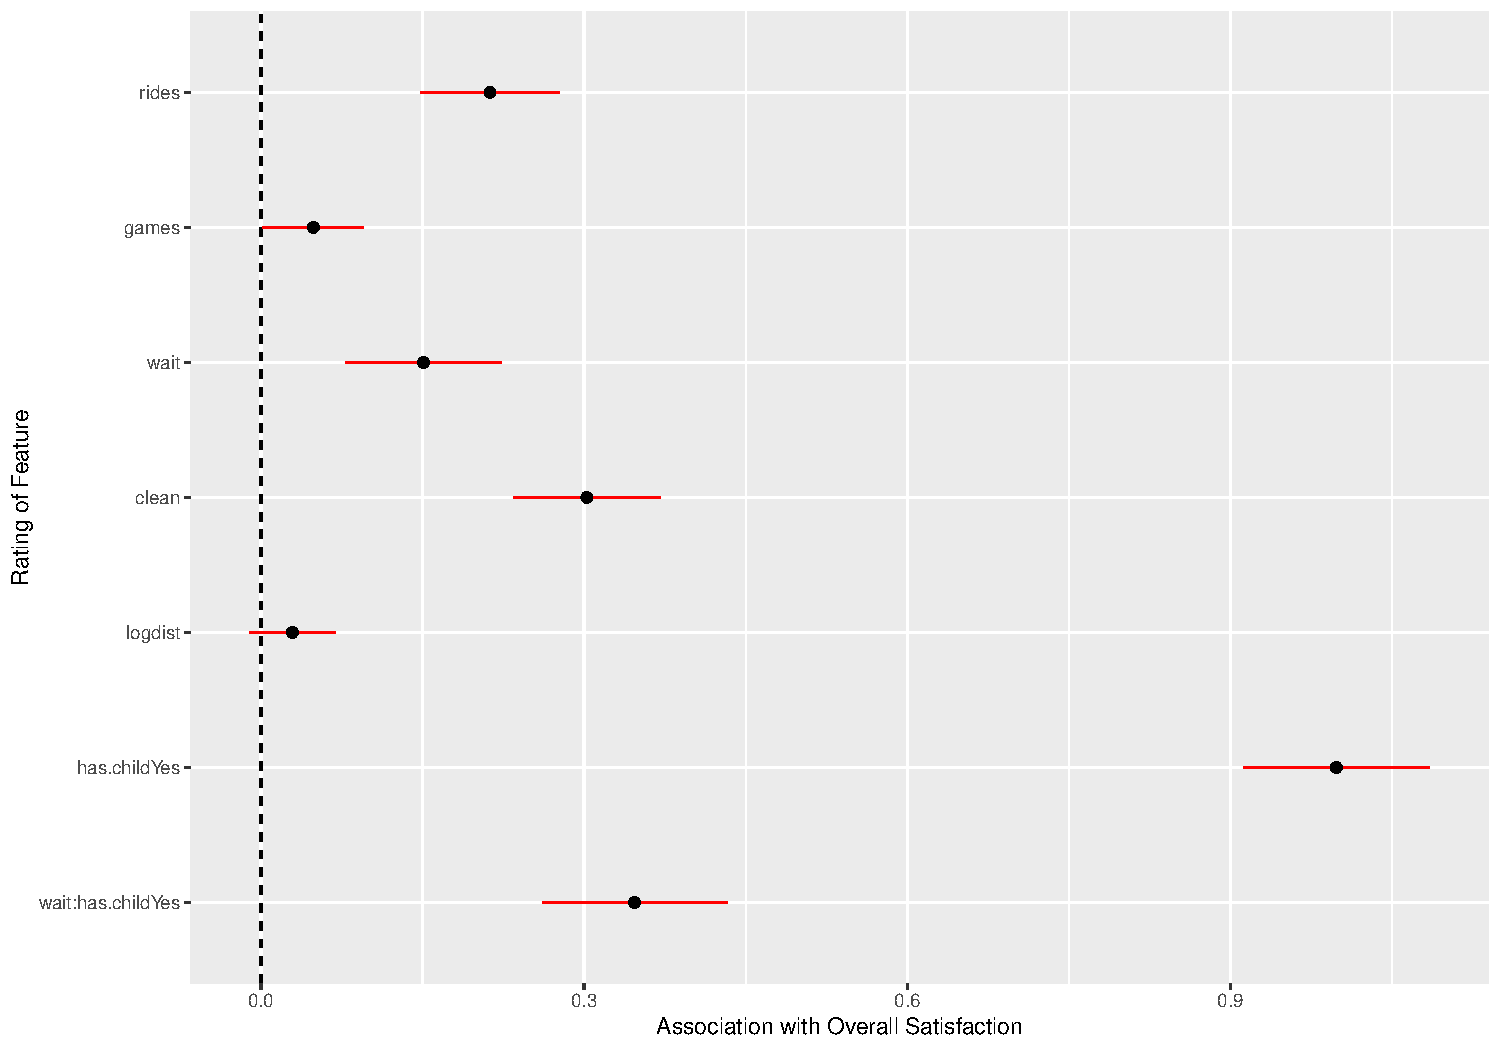
\includegraphics[width=0.5\textwidth,height=\textheight]{007_identifying_drivers_of_outcomes_linear_models_files/figure-beamer/unnamed-chunk-43-1.pdf}
\end{center}
\end{frame}

\begin{frame}[fragile]{}
\phantomsection\label{section-42}
\begin{itemize}
\tightlist
\item
  Formula syntax
\end{itemize}

\begin{table}
\centering\begingroup\fontsize{7}{9}\selectfont

\begin{tabular}[t]{ll}
\toprule
Formula in R & Statistical Model\\
\midrule
y $\sim$ x & $y_i = \beta_0 + \beta_1x_i + \varepsilon_i$\\
y $\sim$ -1 + x & $y_i = \beta_1 x_i + \varepsilon_i$\\
y $\sim$ x + z & $y_i = \beta_0 + \beta_1 x_i + \beta_2 z_i + \varepsilon_i$\\
y $\sim$ x + z + x:z & $y_i = \beta_0 + \beta_1 x_i + \beta_2 z_i + \beta_3 x_i z_i + \varepsilon_i$\\
y $\sim$ x*z & $y_i = \beta_0 + \beta_1 x_i + \beta_2 z_i + \beta_3 x_i z_i + \varepsilon_i$\\
y $\sim$ (x + z + w)$\^{}$2 & $y_i = \beta_0 + \beta_1 x_i + \beta_2 z_i + \beta_3 w_i + \beta_4 x_i z_i + \beta_5 x_i w_i + \beta_6 w_i z_i + \varepsilon_i$\\
y $\sim$ (x + z + w)$\^{}$2 - x:z & $y_i = \beta_0 + \beta_1 x_i + \beta_2 z_i + \beta_3 w_i + \beta_4 x_i w_i + \beta_5 w_i z_i + \varepsilon_i$\\
y $\sim$ x + I(x$^2$) & $y_i = \beta_0 + \beta_1x_i + \beta_1x_i^2 + \varepsilon_i$\\
\bottomrule
\end{tabular}
\endgroup{}
\end{table}

\begin{itemize}
\tightlist
\item
  Try the following models using \texttt{tidy}:
\end{itemize}

\tiny

\begin{Shaded}
\begin{Highlighting}[]
\FunctionTok{lm}\NormalTok{(}\AttributeTok{formula =}\NormalTok{ overall }\SpecialCharTok{\textasciitilde{}}\NormalTok{ rides, }\AttributeTok{data =}\NormalTok{ amusement\_park\_std) }\SpecialCharTok{|\textgreater{}} \FunctionTok{tidy}\NormalTok{()}
\FunctionTok{lm}\NormalTok{(}\AttributeTok{formula =}\NormalTok{ overall }\SpecialCharTok{\textasciitilde{}} \SpecialCharTok{{-}}\DecValTok{1} \SpecialCharTok{+}\NormalTok{ rides, }\AttributeTok{data =}\NormalTok{ amusement\_park\_std) }\SpecialCharTok{|\textgreater{}} \FunctionTok{tidy}\NormalTok{()}
\FunctionTok{lm}\NormalTok{(}\AttributeTok{formula =}\NormalTok{ overall }\SpecialCharTok{\textasciitilde{}}\NormalTok{ rides }\SpecialCharTok{+}\NormalTok{ has.child, }\AttributeTok{data =}\NormalTok{ amusement\_park\_std) }\SpecialCharTok{|\textgreater{}} \FunctionTok{tidy}\NormalTok{()}
\FunctionTok{lm}\NormalTok{(}\AttributeTok{formula =}\NormalTok{ overall }\SpecialCharTok{\textasciitilde{}}\NormalTok{ rides }\SpecialCharTok{+}\NormalTok{ has.child }\SpecialCharTok{+}\NormalTok{ has.child, }\AttributeTok{data =}\NormalTok{ amusement\_park\_std) }\SpecialCharTok{|\textgreater{}} \FunctionTok{tidy}\NormalTok{()}
\FunctionTok{lm}\NormalTok{(}\AttributeTok{formula =}\NormalTok{ overall }\SpecialCharTok{\textasciitilde{}}\NormalTok{ (rides }\SpecialCharTok{+}\NormalTok{ has.child }\SpecialCharTok{+}\NormalTok{ weekend)}\SpecialCharTok{\^{}}\DecValTok{2}\NormalTok{, }
   \AttributeTok{data =}\NormalTok{ amusement\_park\_std) }\SpecialCharTok{|\textgreater{}} \FunctionTok{tidy}\NormalTok{()}
\FunctionTok{lm}\NormalTok{(}\AttributeTok{formula =}\NormalTok{ overall }\SpecialCharTok{\textasciitilde{}}\NormalTok{ (rides }\SpecialCharTok{+}\NormalTok{ has.child }\SpecialCharTok{+}\NormalTok{ weekend)}\SpecialCharTok{\^{}}\DecValTok{2} \SpecialCharTok{{-}}\NormalTok{ rides}\SpecialCharTok{:}\NormalTok{has.child, }
   \AttributeTok{data =}\NormalTok{ amusement\_park\_std) }\SpecialCharTok{|\textgreater{}} \FunctionTok{tidy}\NormalTok{()}
\FunctionTok{lm}\NormalTok{(}\AttributeTok{formula =}\NormalTok{ overall }\SpecialCharTok{\textasciitilde{}}\NormalTok{ rides }\SpecialCharTok{+} \FunctionTok{I}\NormalTok{(rides}\SpecialCharTok{\^{}}\DecValTok{2}\NormalTok{) }\SpecialCharTok{{-}}\NormalTok{ rides}\SpecialCharTok{:}\NormalTok{has.child, }\AttributeTok{data =}\NormalTok{ amusement\_park\_std) }\SpecialCharTok{|\textgreater{}} \FunctionTok{tidy}\NormalTok{()}
\end{Highlighting}
\end{Shaded}
\end{frame}

\section{Acknowledgments}\label{acknowledgments}

\begin{frame}{}
\phantomsection\label{section-43}
\begin{itemize}
\item
  To my family that supports me
\item
  To the taxpayers of Colombia and the
  \href{https://www.umng.edu.co/estudiante}{\textbf{UMNG students}} who
  pay my salary
\item
  To the \href{https://www.business-science.io/}{\textbf{Business
  Science}} and \href{https://www.rfordatasci.com/}{\textbf{R4DS Online
  Learning}} communities where I learn
  \href{https://www.r-project.org/about.html}{\textbf{R}} and
  \href{https://www.python.org/about/}{\textbf{\(\pi\)-thon}}
\item
  To the \href{https://www.r-project.org/contributors.html}{\textbf{R
  Core Team}}, the creators of
  \href{https://posit.co/products/open-source/rstudio/}{\textbf{RStudio
  IDE}}, \href{https://quarto.org/}{\textbf{Quarto}} and the authors and
  maintainers of the packages
  \href{https://CRAN.R-project.org/package=tidyverse}{\textbf{tidyverse}},
  \href{https://CRAN.R-project.org/package=skimr}{\textbf{skimr}},
  \href{https://CRAN.R-project.org/package=tidymodels}{\textbf{tidymodels}},
  \href{https://CRAN.R-project.org/package=dotwhisker}{\textbf{dotwhisker}},
  \href{https://CRAN.R-project.org/package=kableExtra}{\textbf{kableExtra}}
  and
  \href{https://CRAN.R-project.org/package=tinytex}{\textbf{tinytex}}
  for allowing me to access these tools without paying for a license
\item
  To the \href{https://www.kernel.org/category/about.html}{\textbf{Linux
  kernel community}} for allowing me the possibility to use some
  \href{https://static.lwn.net/Distributions/}{\textbf{Linux
  distributions}} as my main
  \href{https://en.wikipedia.org/wiki/Operating_system}{\textbf{OS}}
  without paying for a license
\end{itemize}
\end{frame}

\section*{References}\label{references}
\addcontentsline{toc}{section}{References}

\begin{frame}[allowframebreaks]{References}
\phantomsection\label{refs}
\begin{CSLReferences}{1}{0}
\bibitem[\citeproctext]{ref-chapman_r_2019}
Chapman, Chris, and Elea McDonnell Feit. 2019. \emph{R {For} {Marketing}
{Research} and {Analytics}}. 2nd ed. 2019. Use {R}! Cham: Springer
International Publishing : Imprint: Springer.
\url{https://doi-org.ezproxy.umng.edu.co/10.1007/978-3-030-14316-9}.

\end{CSLReferences}
\end{frame}




\end{document}
